

\documentclass[11pt,a4paper,twoside]{book}

\newcommand{\ficherosBasicosTeXiS}{%
TeXiS/TeXiS_pream,TeXiS/TeXiS_cab,TeXiS/TeXiS_bib,TeXiS/TeXiS_cover,%
TeXiS/TeXiS_part%
}
\newcommand{\compilaCapitulo}[1]{%
\includeonly{\ficherosBasicosTeXiS,\ficherosBasicosTexto,Capitulos/#1}%
}

\newcommand{\compilaApendice}[1]{%
\includeonly{\ficherosBasicosTeXiS,\ficherosBasicosTexto,Apendices/#1}%
}

\include{config}

% Paquete de la plantilla
\usepackage{TeXiS/TeXiS}
\usepackage{svg}
\usepackage{amsmath}
\usepackage{wrapfig}
\usepackage{array}
\usepackage{float}
\restylefloat{table}
\usepackage{pgfplots}
\usepackage{amssymb}
\usepackage{tikz}
\usepackage{hyperref}
\hypersetup{
  citebordercolor=red,
  filebordercolor=red,
  linkbordercolor=red,
urlbordercolor=red
}
\urlstyle{same}


\usepackage{natbib}
\bibliographystyle{humannat}


% Incluimos el fichero con comandos de constantes
\include{constantes}
% Sacamos en el log de la compilaci�n el copyright
\typeout{Copyright Pablo G\'omez Calvo y Sergio J. Higuera Velasco}

%
% "Metadatos" para el PDF
%
\ifpdf\hypersetup{%
    pdftitle = {Control Remoto de Videojuegos con Smartphones},
    pdfsubject = {Memoria TFG},
    pdfkeywords = {Plantilla, LaTeX, TFG, UCM, Videojuegos},
    pdfauthor = {\textcopyright\ \autor},
    pdfcreator = {\LaTeX\ con el paquete \flqq hyperref\frqq},
    pdfproducer = {pdfeTeX-0.\the\pdftexversion\pdftexrevision},
    }
    \pdfinfo{/CreationDate (\today)}
\fi


%- - - - - - - - - - - - - - - - - - - - - - - - - - - - - - - - - - -
%                        Documento
%- - - - - - - - - - - - - - - - - - - - - - - - - - - - - - - - - - -
\begin{document}


% Incluimos el  fichero de definici�n de guionado  de algunas palabras
% que LaTeX no ha dividido como deber�a
\input{guionado}

% Marcamos  el inicio  del  documento para  la  numeraci�n de  p�ginas
% (usando n�meros romanos para esta primera fase).
\frontmatter

\include{Cascaras/cover}

\include{Cascaras/dedicatoria}

%---------------------------------------------------------------------
%
%                      agradecimientos.tex
%
%---------------------------------------------------------------------
%
% agradecimientos.tex
% Copyright 2009 Marco Antonio Gomez-Martin, Pedro Pablo Gomez-Martin
%
% This file belongs to the TeXiS manual, a LaTeX template for writting
% Thesis and other documents. The complete last TeXiS package can
% be obtained from http://gaia.fdi.ucm.es/projects/texis/
%
% Although the TeXiS template itself is distributed under the 
% conditions of the LaTeX Project Public License
% (http://www.latex-project.org/lppl.txt), the manual content
% uses the CC-BY-SA license that stays that you are free:
%
%    - to share & to copy, distribute and transmit the work
%    - to remix and to adapt the work
%
% under the following conditions:
%
%    - Attribution: you must attribute the work in the manner
%      specified by the author or licensor (but not in any way that
%      suggests that they endorse you or your use of the work).
%    - Share Alike: if you alter, transform, or build upon this
%      work, you may distribute the resulting work only under the
%      same, similar or a compatible license.
%
% The complete license is available in
% http://creativecommons.org/licenses/by-sa/3.0/legalcode
%
%---------------------------------------------------------------------
%
% Contiene la p�gina de agradecimientos.
%
% Se crea como un cap�tulo sin numeraci�n.
%
%---------------------------------------------------------------------

\chapter{Agradecimientos}

\cabeceraEspecial{Agradecimientos}

\begin{FraseCelebre}
\begin{Frase}
Nadie es innecesario.
\end{Frase}
\begin{Fuente}
Yit\'an, Final Fantasy IX
\end{Fuente}
\end{FraseCelebre}

El primer agradecimiento hay que darselo a la Universidad Complutense por aceptar la creaci\'on de este grado, un grado que demuestra la importancia del mundo de los videojuegos en la sociedad actual. Con este grado se han conseguido romper muchas barreras, entre ellas est\'a poder especializarse y adoptar los videojuegos como nuestra profesi\'on, y tras 4 a\~nos podemos decir que no ha sido f\'acil, pero somos ingenieros y desarrolladores de videojuegos.
\\
\\
Dar gracias a los profesores que nos han acompa\~nado estos a\~nos y que han contribuido en el desarrollo del grado. Una menci\'on aparte para las dos personas que han hecho posible la realizaci\'on de este Trabajo de Fin de Grado, Carlos Le\'on Aznar y Pedro Pablo G\'omez Mart\'in.
\\
\\
Nuestro \'ultimo  agradecimiento va dirigido a nuestras familias. No ha sido f\'acil aguantar las noches de desvelo, alegr\'ias y enfados tras estos 4 a\~nos en la universidad.
\\

\endinput
% Variable local para emacs, para  que encuentre el fichero maestro de
% compilaci�n y funcionen mejor algunas teclas r�pidas de AucTeX
%%%
%%% Local Variables:
%%% mode: latex
%%% TeX-master: "../Tesis.tex"
%%% End:


%---------------------------------------------------------------------
%
%                      resumenManual.tex
%
%---------------------------------------------------------------------
%
% resumenManual.tex
% Copyright 2009 Marco Antonio Gomez-Martin, Pedro Pablo Gomez-Martin
%
% This file belongs to the TeXiS manual, a LaTeX template for writting
% Thesis and other documents. The complete last TeXiS package can
% be obtained from http://gaia.fdi.ucm.es/projects/texis/
%
% Although the TeXiS template itself is distributed under the 
% conditions of the LaTeX Project Public License
% (http://www.latex-project.org/lppl.txt), the manual content
% uses the CC-BY-SA license that stays that you are free:
%
%    - to share & to copy, distribute and transmit the work
%    - to remix and to adapt the work
%
% under the following conditions:
%
%    - Attribution: you must attribute the work in the manner
%      specified by the author or licensor (but not in any way that
%      suggests that they endorse you or your use of the work).
%    - Share Alike: if you alter, transform, or build upon this
%      work, you may distribute the resulting work only under the
%      same, similar or a compatible license.
%
% The complete license is available in
% http://creativecommons.org/licenses/by-sa/3.0/legalcode
%
%---------------------------------------------------------------------
%
% Contiene el cap�tulo del resumen.
%
% Se crea como un cap�tulo sin numeraci�n.
%
%---------------------------------------------------------------------


\chapter{Resumen}
\cabeceraEspecial{Resumen}

\begin{FraseCelebre}
\begin{Frase}
\textexclamdown No est\'ais preparados!
\end{Frase}
\begin{Fuente}
 Illidan Tempestira, World of Warcraft
\end{Fuente}
\end{FraseCelebre}

Los videojuegos pueden ser disfrutados con una amplia variedad de dispositivos de entrada. Desde un mando tradicional hasta unas gafas de realidad virtual pasando por estaciones de simulaci\'on de conducci\'on de coches. Los dispositivos m\'oviles no se quedan atr\'as en ofrecer nuevas posibilidades para jugar a videojuegos. La presencia de estos dispositivos en gran parte de los hogares hace que estos se conviertan en una alternativa a los dispositivos de entrada habituales. Por ello, este proyecto tiene como objetivo la utilizaci\'on de un dispositivo m\'ovil como dispositivo de entrada de juegos ejecutados en el pc. Para ello se ha desarrollado una librer\'ia para el motor de videojuegos Unity y una aplicaci\'on para Android. \\

La herramienta desarrollada se ha probado en un juego para comprobar la usabilidad de la herramienta y su proceso de inclusi\'on. Con este juego se han realizado pruebas de rendimiento para comprobar la velocidad del proceso y ver si la librer\'ia cumpl\'ia los est\'andares de tasas de fotogramas por segundo. Los resultados muestran que este est\'andar es alcanzado por los dispositivos en los que se ha probado.

\addvspace{1cm}


\Large{\textbf{Palabras claves}}
\normalsize

\addvspace{1cm}

Dispositivo de entrada, m\'ovil, Android, Unity, videojuego, desarrollo de videojuegos


\chapter{Abstract}

\huge{\textbf{Keywords}}
\normalsize
\endinput
% Variable local para emacs, para  que encuentre el fichero maestro de
% compilaci�n y funcionen mejor algunas teclas r�pidas de AucTeX
%%%
%%% Local Variables:
%%% mode: latex
%%% TeX-master: "../ManualTeXiS.tex"
%%% End:


\ifx\generatoc\undefined
\else
\include{TeXiS/TeXiS_toc}
\fi

% Marcamos el  comienzo de  los cap�tulos (para  la numeraci�n  de las
% p�ginas) y ponemos la cabecera normal
\mainmatter
\restauraCabecera

%\include{Capitulos/Parte1}
%---------------------------------------------------------------------
%
%                          Cap�tulo 1
%
%---------------------------------------------------------------------
%Cambios en esta versión:
% Primer párrafo de introducción.
%---------------------------------------------------------------------

\chapter{Introducci\'on}

La tecnolog\'ia se ha vuelto indispensable en pr\'acticamente todos los \'ambitos de nuestra sociedad. Son pocos los escenarios  en los que no se vea involucrado un aparato tecnol\'ogico. Tareas tan cotidianas como preparar un caf\'e por la ma\~nana o levantar una persiana ahora son posibles con una aplicaci\'on en nuestro m\'ovil o con un comando por voz. \\

Adem\'as de para mejorar nuestras tareas, los dispositivos m\'oviles se han unido a los ordendores y las consolas de videojuegos en la tarea de entretener a una gran cantidad de usuarios. Con la progresi\'on en la calidad de los dispositivos m\'oviles, la industria del videojuego ha decidido unirse y comenzar a lanzar juegos con grandes presupuestos al mercado m\'ovil. \\

En los \'ultimos a\~nos las compa\~nias de videojuegos han encontrado en los dispositivos m\'oviles un aliado, no solamente para vender videojuegos sino para ser utilizados como accesorios de las consolas y los ordenadores. \\


Con este proyecto se pretende explorar la situaci\'on actual del uso de dispositivos m\'oviles como dispositivo de entrada para videojuegos y las motivaciones que existen para invertir e investigar en este nuevo modelo de interacci\'on de usuario. Junto con esta investigaci\'on, se llevar\'a a cabo con un proceso de desarrollo de una herramienta que haga posible jugar utilizando un dispositivo m\'ovil como dispositivo de entrada para videojuegos.


%-------------------------------------------------------------------
\section{Motivaci\'on}
%-------------------------------------------------------------------

Uno de los pilares que siempre han caracterizado a la industria del videojuego es la innovaci\'on a la hora de crear nuevas experiencias para los usuarios. Experiencias que enriquecen a muchos jugadores y que cada vez es disfrutable de una manera m\'as c\'omoda y flexible. Uno de los culpables del aumento de esta flexibilidad a la hora de jugar son los dispositivos m\'oviles. \\

En esta \'ultima d\'ecada el mercado del \textit{gaming} ha acogido al tel\'efono m\'ovil como su nuevo integrante. Los juegos para m\'oviles han tenido mucho \'exito entre las nuevas generaciones de jugadores, tanto, que los fabricantes de m\'oviles han comenzado a lanzar dispositivos que se enfocan directamente en el mundo de los videojuegos. \citet{moviles} plantea si estos nuevos dispositivos m\'oviles son una amenza para las consolas actuales y presenta el caso de varios fabricantes de perif\'ericos \textit{gaming} que se han lanzado al mundo de la fabricaci\'on de \textbf{smartphones} orientados a jugar. \\

T\'itulos relevantes dentro de la industria como \textit{League of Legends}, \textit{Call of Duty} o \textit{Fortnite} ya tienen su versi\'on para dispositivos m\'oviles. Gracias a que estos t\'itulos son gratuitos y se encuentran a la cabeza de los \textit{e-sports} en sus modalidades de PC y consola, su relevancia dentro de las plataformas m\'oviles ha sido aun mayor. A pesar de esto, tal y como cuenta \cite{futuro} en un art\'iculo, existen varios limitantes en el \textit{gaming} para dispositivos m\'oviles. Algunos de estos limitantes son la bateria de los dispositivos y la necesidad de una conexi\'on estable a internet.\\

Teniendo en cuenta estos inconvenientes, 3 de las compa\~n\'ias m\'as relevantes en el mundo de los videojuegos: Sony, Microsoft y Nintendo, han apostado por el uso de los dispositivos m\'oviles como complemento para sus consolas. Nintendo por su parte ha desarrollado aplicaciones\footnote{Aplicaciones Nintendo - \url{https://www.nintendo.es/Familia-Nintendo-Switch/Nintendo-Switch-Online/Aplicacion-para-moviles-1374628.html}} para llevar a cabo la comunicaci\'on en sus juegos online. Estas aplicaciones suplen la falta de micr\'ofono incorporado en la consola y permite seguir utilizando el chat de voz cuando la consola se encuentra conectada al dock. Microsoft ha desarrollado una aplicaci\'on con la que poder jugar de manera remota a su consola. Gracias a esta aplicaci\'on, el usuario puede descargarse los juegos en su Xbox\footnote{ Remote Controller XBOX - \url{https://www.xbox.com/es-ES/consoles/remote-play}}, ejecutarlos y conectar su m\'ovil o tablet para poder jugar directamente en su smartphone a trav\'es de internet. Al igual que Microsoft, Sony tambi\'en ha desarrollado su aplicaci\'on para poder jugar de manera remota a PlayStation 4 y PlayStation 5, \textbf{PS Remote Play\footnote{PS Remote Play - \url{https://remoteplay.dl.playstation.net/remoteplay/lang/es/index.html}}}. Adem\'as de para poder jugar, Sony ha desarrollado otra aplicaci\'on que permite a los usuarios controlar la interfaz de la consola desde su dispositivo m\'ovil haciendo que este simule ser un mando y una segunda pantalla (\textbf{PS4 Second Screen\footnote{PS4 Second Screen - \url{https://play.google.com/store/apps/details?id=com.playstation.mobile2ndscreen&hl=es&gl=US}}}).\\

Despu\'es de desarrollar sus aplicaciones, Sony sac\'o al mercado una serie de juegos conocidos como \textbf{PlayLink\footnote{PlayLink - \url{https://www.playstation.com/es-es/accessories/playlink/}}}. Este nuevo tipo de juegos se concentran en una colecci\'on de t\'itulos que tienen una caracter\'istica com\'un, no es necesario usar un mando convencional de PlayStation. Estos t\'itulos se juegan directamente usando el tel\'efono m\'ovil como mando y el \'unico requisito es tener cada uno de los dispositivos m\'oviles conectados a la consola via Wi-Fi. Esto soluciona por completo el problema de la escasez de mandos de consola en los hogares ya que \'unicamente ser\'an necesarios los tel\'efonos m\'oviles de las personas que vayan a jugar.\\

El prop\'osito de este trabajo consiste en lograr utilizar un m\'ovil como dispositivo de entrada en un juego de PC. Para poder lograrlo, se propone crear una herramienta libre para el motor de videojuegos Unity y posteriormente subirla a la tienda de Unity, Unity Asset Store\footnote{Unity Asset Store - \url{https://assetstore.unity.com/}}. Esto permitir\'a la posibilidad de ampliaci\'on y modificaci\'on de la herramienta dependiendo de las necesidades de cada usuario.


\section{Objetivos}

La finalidad del proyecto es la conexi\'on entre 2 dispositivos, uno de ellos ejecuta el juego y el otro funciona como un dispositivo de entrada / mando para controlar el videojuego. Esta conexi\'on debe ser estable, con el m\'inimo \textit{Input Lag} posible y que sea f\'acil de incorporar en proyectos ya estructurados.\\

El m\'ovil, que funcionar\'ia como dispositivo de entrada, recibe im\'agenes del PC, dispositivo donde se ejecuta el juego, para as\'i mostrarle al usuario una im\'agen de un mando virtual en su pantalla. Una vez el usuario interactue con este mando virtual, las pulsaciones de los botones que se encuentran en la pantalla se envian al juego a modo de entrada de usuario.\\

Con respecto a las plataformas donde realizar ambas aplicaciones, hemos decidido utilizar Android de manera nativa para el dispositivo de entrada y Unity para la parte del juego. Se ha decidido hacer el plug-in para Unity ya que es uno de los motores de juegos m\'as utilizado actualmente. El uso de Android para la aplicaci\'on de m\'ovil se debe a las facilidades que ofrece Google para subir aplicaciones a la plataforma Play Store y al amplio parque de dispositivos Android que existen actualmente.\\

Para conseguir este objetivo se ha divido el objetivo final en los siguientes pasos:

\begin {itemize}
\item Desarrollar y publicar un \textit{plug-in open source} para Unity que permita establecer conexi\'on y recibir \textit{input} desde otro dispositivo.
\item Desarrollar y publicar una aplicaci\'on \textit{open source} para Android que permita establecer conexi\'on con otro dispositivo para ser usado como dispositivo de entrada.
\item Evidenciar y realizar un estudio posterior de los resultados del proyecto atrav\'es de una serie de pruebas con usuarios. 
\end {itemize}

Para confirmar que las aplicaciones desarrolladas funcionan, se va a realizar una prueba de concepto y una posterior prueba con usuarios para obtener una serie de datos como latencia de red, uso del procesador y tiempos de compresi\'on y descompresi\'on de im\'agenes. Tras recolectar estos datos y analizarlos, se podr\'a llegar a una conclusi\'on positiva si la herramienta funciona y la latencia no es apreciable o si por el contrario hubiese mucha latencia y no funcionase de manera fluida las conclusiones ser\'ian negativas.

\section{Metodolog\'ia}

Como metodolog\'ia de desarrollo se ha decidido usar una metodolog\'ia \'agil de producci\'on que es habitual en la industria del desarrollo de software y videojuegos. Se ha elegido una metodolog\'ia \'agil por la experiencia positiva en proyectos previos.

\textbf{Scrum}, propuesto por \cite{scrum} and Sutherland (1995), es un framework para la gesti\'on de proyectos de trabajo en equipo. El paradigma se basa en un principio simple: comenzar con metas a corto plazo que formen parte del resultado final, tras esto se sigue el progreso y modifica seg\'un se avance en el proyecto. Scrum adem\'as de realizar reunionen diarias, refleja la separaci\'on del tiempo total de trabajo en hitos (conocidos como \textit{Sprint}). Estos \textit{sprints} suelen realizarse cada mes para crear consistencia y cuyo objetivo es incrementar el valor del producto en el que se est\'a trabajando.

Debido a los problemas de disponibilidad durante el desarrollo del proyecto, se realizaba una peque\~na reuni\'on de 10 minutos cada 1-3 d\'ias para ver el progreso de cada uno de los integrantes. En estas reuniones se revisaba la planificaci\'on para la siguiente reuni\'on o la siguiente semana. Al principio del desarrollo fueron necesarias reuniones mucho m\'as largas que en muchas ocasiones incluian a los directores del TFG en las que se discut\'ian las diferentes caracter\'isticas que deber\'ian tener las aplicaciones que se estaban desarrollando. Estas reuniones m\'as extensas serv\'ian como cierre de \textit{Sprint} y como preparaci\'on del siguiente. El seguimiento de las diferentes tareas a realizar se realizaba usando la herramienta online \textbf{Pivotal Tracker} donde se marcaban las tareas con 3 posibles estados: ``Open'', ``In Progress'' o ``Done''.


\section{Planificaci\'on}

La planificaci\'on del desarrollo de este proyecto se ha dividido en 3 fases:\\


\textbf{Documentaci\'on y dise\~no:} Durante esta fase tratamos de delimitar claramente el alcance y objetivos del TFG, reunir fuentes y referencias y preparar las herramientas que se utilizar\'ian durante el resto del desarrollo. Adem\'as, en esta primera fase se realiz\'o un dise\~no de las aplicaciones que se desarrollar\'ian en los meses posteriores.\\

\textbf{Desarrollo:} Durante esta fase del desarrollo se realizaron todas las funcionalidades especificadas en la fase anterior del proyecto. Al hacerse revisiones peri\'odicas de la implementaci\'on, algunas de las funcionalidades iniciales sufrieron cambios o fueron eliminidas y se a\~nadieron otras que encajaban m\'as con el rumbo que estaba tomando el desarrollo. 
Esta fase ha ocupado la mayor parte del tiempo que ha tomado realizar este proyecto. Durante esta fase se realizaron 2 aplicaciones en forma de demo con las que poder probar la herramienta y demostrar la viabilidad del proyecto.\\

\textbf{Cierre:} Durante la fase final del desarrollo se realizaron las mejoras finales de las aplicaciones y se refinaron los \'ultimos detalles de rendimiento. En esta fase tambi\'en se realizaron las pruebas con usuarios para extraer datos tanto de rendimiento de las aplicaciones como de posibles fallos y mejoras de las aplicaciones. Estos datos se han refinado, filtrado y analizado y han servido para extraer las conclusiones finales de este trabajo. Adem\'as, durante esta \'ultima fase del desarrollo se ha trabajado en terminar la redacci\'on de este documento junto con la revisi\'on por los directores de este TFG. 

\section{Estructura del documento}

Este proyecto se divide en 6 cap\'itulos, cada uno de ellos dedicado a una tem\'atica. Esta secci\'on est\'a situada en el cap\'itulo de introducci\'on donde se ha definido la motivaci\'on y los objetivos del proyecto.\\

El cap\'itulo 2 recoge el estudio inicial del estado del arte en el cual se exponen los antecedentes de la tem\'atica del proyecto. En este cap\'itulo se mencionan y explican los cambios que han sufrido los diferentes dispositivos de entrada para videojuegos desde los inicios. En este cap\'itulo se incluye tambi\'en el funcionamiento de los sistemas de streaming y la retroalimentaci\'on en los controladores de videojuegos.\\

En el cap\'itulo 3 se explica todo lo relacionado con la especificaci\'on de las aplicaciones que se van a desarrollar. Esta especificaci\'on incluye una descripci\'on del protocolo de comunicaci\'on entre dispositivos necesario para este proyecto.\\

En el cap\'itulo 4 se explica de manera detallada la implementaci\'on de las aplicaciones que se han desarrollado para este proyecto.\\

El cap\'itulo 5 se explica la demo desarrollada para probar la viabilidad del \textit{plug-in} desarrollado y como caso pr\'actico para la presentaci\'on de este proyecto. Adem\'as, se recopila el peque\~no experimento que se ha llevado a cabo con diferentes usuarios para probar la aplicaci\'on y recopilar \textit{feedback} de los diferentes usuarios que han probado la demo. Tambi\'en se describen los participantes, los resultados obtenidos y la discusi\'on sobre estos resultados.\\

En el \'ultimo cap\'itulo se explican de manera detalla las conclusiones obtenidas despu\'es de realizar el proyecto y una visi\'on general del trabajo futuro que inspira este proyecto.



%El manual tiene, por �ltimo, un ap�ndice que, si bien no es
%interesante desde el punto de vista del usuario, nos sirve de excusa
%para proporcionar el c�digo \LaTeX\ necesario para su creaci�n: a modo
%de ``as� se hizo'', comenta brevemente c�mo fue el proceso de
%escritura de nuestras tesis.



% Variable local para emacs, para  que encuentre el fichero maestro de
% compilaci�n y funcionen mejor algunas teclas r�pidas de AucTeX
%%%
%%% Local Variables:
%%% mode: latex
%%% TeX-master: "../ManualTeXiS.tex"
%%% End:

%---------------------------------------------------------------------
%
%                          Cap�tulo 2
%
%---------------------------------------------------------------------
%
% 02EstructuraYGeneracion.tex
% Copyright 2009 Marco Antonio Gomez-Martin, Pedro Pablo Gomez-Martin
%
% This file belongs to the TeXiS manual, a LaTeX template for writting
% Thesis and other documents. The complete last TeXiS package can
% be obtained from http://gaia.fdi.ucm.es/projects/texis/
%
% Although the TeXiS template itself is distributed under the 
% conditions of the LaTeX Project Public License
% (http://www.latex-project.org/lppl.txt), the manual content
% uses the CC-BY-SA license that stays that you are free:
%
%    - to share & to copy, distribute and transmit the work
%    - to remix and to adapt the work
%
% under the following conditions:
%
%    - Attribution: you must attribute the work in the manner
%      specified by the author or licensor (but not in any way that
%      suggests that they endorse you or your use of the work).
%    - Share Alike: if you alter, transform, or build upon this
%      work, you may distribute the resulting work only under the
%      same, similar or a compatible license.
%
% The complete license is available in
% http://creativecommons.org/licenses/by-sa/3.0/legalcode
%
%---------------------------------------------------------------------

\chapter{Estado del arte en entrada de usuario para videojuegos}
\label{cap2}


A lo largo de las diferentes generaciones de computadores y de consolas se han ido desarrollando una serie de dispositivos de entrada que permiten al usuario interactuar con la m\'aquina. Estos dispositivos van desde teclados y ratones hasta c\'amaras que permiten transformar tus movimientos f\'isicos en movimientos dentro de un entorno virtual pasando por detectores de aceleraci\'on y pantallas t\'actiles. En este cap\'itulo se presentan muchos de los trabajos pasados en el \'ambito de los dispositivos de entrada de usuario.
%-------------------------------------------------------------------
\section{Dispositivos de entrada en ordenadores de prop\'osito general}

Los dispositivos de entrada son aquellos que permiten introducir datos o informaci\'on en un ordenador para que este los procese u ordene. Otro t\'ermino usado para estos dispositivos es perif\'erico. A pesar de que este t\'ermino implica a menudo el concepto de adicional y no esencial, en muchos sistemas inform\'aticos son elementos fundamentales. \cite{entradasalida} expone que los m\'as comunes de estos dispositivos de entrada son el teclado y rat\'on. Pero no existen \'unicamente estos 2 dispositivos de entrada, a lo largo de la historia de la inform\'atica se han ido desarrollando diversos dispositivos de entrada tanto sonora como visual y de movimiento mec\'anico.\\

\subsection{Evoluci\'on de los teclados}

La historia de los teclados actuales tiene su origen en las m\'aquinas de escribir. Estas primeras m\'aquinas de escribir tienen su origen en el a\~no 1877, cuando la empresa Remington comenz\'o a comercializar de manera masiva las m\'aquinas de escribir. En un primer momento las teclas de dispusieron en orden alfab\'etico, algo que cambiar\'ia un a\~no despu\'es con la aparici\'on de la primera patente del teclado QWERTY. Tal y como se\~nala \cite{jimmy} en su art\'iculo, esta primera versi\'on de las m\'aquinas de escribir ten\'ian un defecto que fue notorio cuando los usuarios escrib\'ian r\'apidamente una sucesi\'on de letras que se encontraban cerca en el teclado. Este defecto consist\'ia en que las barras que conectaban cada una de las teclas chocaban si se pulsaban teclas que estuvieran demasiado cerca.  Para evitar este fallo en el modelo inicial se desarroll\'o el sistema QWERTY, el cual distancia los pares de letras que se suelen escribir juntas.\\

Uno de los primeros avances de estas m\'aquinas de escribir ocurri\'o en la d\'ecada de 1930, cuando se combinaron la tecnolog\'ia de la entrada e impresi\'on de las m\'aquinas de escribir con la tecnolog\'ia de la comunicaci\'on del tel\'egrafo. Este dispositivo fue muy popular durante el siglo XX y sus funciones eran las de enviar y recibir mensajes mecanografiados de un punto a otro a trav\'es de un canal de comunicaci\'on. M\'as adelante fue utilizado en conjunto con las cintas perforadas para almacenar datos en los primeros ordenadores. As\'i, en 1955, el Whirlwind del MIT, se convierte en el primer ordenador del mundo que permite a sus usuarios introducir comandos a trav\'es de un teclado. Adem\'as confirm\'o lo \'util y conveniente que puede ser un dispositivo de entrada como el teclado.\\

Actualmente las principales mejoras que han sufrido los teclados de ordenador se basan en la eliminaci\'on de cables gracias al Bluetooth, la disminuci\'on de la presi\'on que hay que ejercer sobre la tecla para que esta sea detectada y la ergonom\'ia. Con la llegada de los dispositivos t\'actiles se a\~nadi\'o adem\'as el concepto de teclado virtual. Este teclado virtual elimina el uso de un teclado hardware para pasar a un teclado software que imita el teclado tradicional QWERTY pero en una pantalla t\'actil. \\

\subsection{Evoluci\'on de los ratones}

Adem\'as del teclado, el segundo dispositivo de entrada por excelencia es el rat\'on. La primera maqueta [\ref{Fig:primerraton}] fue dise\~nada durante los a\~nos 60, dispon\'ia de 2 ruedas met\'alicas que al desplazarse por una superficie mov\'ian 2 ejes. Cada uno de estos ejes controlaba el movimiento tanto vertical como horizontal del cursor en la pantalla y dispon\'ia de un bot\'on en la parte superior con el que se permit\'ia hacer clic en la posici\'on en la que se encontraba el cursor.\\

\begin{figure}[h]
\centering
\includegraphics[width=0.29\textwidth]{./Imagenes/Bitmap/Primer_raton.jpg}
\caption{Primer rat\'on desarrollado por Douglas Engelbart y Bill English}
\label{Fig:primerraton}
\end{figure}

El siguiente avance del dispositivo fue cambiar su carcasa de madera por una de pl\'astico y a\~nadir m\'as botones. Tal y como describi\'o \cite{xerox} en su art\'iculo, este avance suele ser atribuido a Microsoft o a Apple. Lejos de ser as\'i, fue la empresa \textbf{Xerox} la que realiz\'o el nuevo dise\~no del rat\'on [\ref{Fig:xerox}] y del que es considerado el primer ordenador personal de la historia junto al Altair 8080. Este nuevo dispositivo sustitu\'ia las 2 ruedas que marcaban la posici\'on del cursor por una \'unica bola de metal. La posici\'on relativa de esta bola era la que determinaba la posici\'on del cursor en la pantalla. 

\begin{figure}[!htb]
\begin{minipage}{0.9\textwidth}
    \centering
    \includegraphics[width=0.40\textwidth]{./Imagenes/Bitmap/mouse_xerox_alto(1).png}
    \includegraphics[width=0.20\textwidth]{./Imagenes/Bitmap/mouse_xerox_alto(2).jpg}
\end{minipage}
    \caption{Rat\'on del Xerox Alto de los a\~nos 70}
\label{Fig:xerox}
\end{figure}

En el a\~no 1992 Microsoft decidi\'o vender en un mismo paqueta su \'ultima versi\'on de MS-DOS y Windows 3.1, lo que hizo que el rat\'on pasase a ser un perif\'erico fundamental ya que se dejaba atr\'as el mundo del texto y se abr\'ian a todos los p\'ublicos las interfaces gr\'aficas del PC. Este cambio hizo que el rat\'on siguiera evolucionando y durante la d\'ecada de los 90 e inicios del 2000 los ratones sufrieron algunas mejoras. Algunas de estas mejoras son: una rueda central o lateral para el desplazamiento, el sensor de movimiento \'optico por diodo led o un sensor basado en un l\'aser no visible. Un sector que aprovech\'o mucho esta estandarizaci\'on del rat\'on y de las interfaces gr\'aficas fue el de los videojuegos. El rat\'on se ha convertido en una parte esencial del mundo de los videojuegos de PC, sirviendo no solo para seleccionar y accionar objetos en pantalla en juegos de estrategia, sino para controlar la c\'amara o cambiar la direcci\'on del personaje en juegos de primera y tercera persona.\\

\section{Evoluci\'on de los gamepads a trav\'es de las generaciones de consolas}

Los videojuegos de PC fueron, son y ser\'an muy importantes para el desarrollo de la industria pero las precursoras de este existo son sin dudas las m\'aquinas recreativas. Se dice que el primer intento de videojuego es una patente de 1947 sobre la simulaci\'on del lanzamiento de misiles pero no fue hasta 1958 y la salida del famoso ``Tenis para Dos'' creado por William Higginbotham que se puede comenzar a hablar de videojuegos \citep{tenispara2}. En este juego se recreaba una pista de tenis en la que la pelota iba de un lado a otro de la pista. Poco despu\'es, en 1962 vio la luz \textbf{Spacewar!}. Este t\'itulo fue desarrollado por Steve Russell y posteriormente modificado por sus estudiantes. En este juego lo que se quer\'ia era simular una pelea entre 2 naves en el espacio, fue el primer paso de los juegos multijador en un mismo dispositivo. El dispositivo de entrada de este juego consist\'ia de 2 ejes de rotaci\'on que se usaban para controlar la rotaci\'on y el empuje de la nave. Adem\'as de esto, el mando dispon\'ia de un bot\'on para dispar misiles [\ref{Fig:spacewar}].\\

Ser\'a en la d\'ecada de los 70 cuando las m\'aquinas recreativas comiencen a tener repercusi\'on con la salida de \textbf{Pong} en 1972 y \textbf{Space Invaders} en 1978. Muchos t\'itulos y sagas tienen su inicio en esta \'epoca en la que las salas de recreativas estaban abarrotadas de j\'ovenes dispuestos a pasar all\'i todas las horas posibles jugando y compitiendo con otros jugadores. La salida de las consolas, las r\'apidas mejoras del hardware y el avance la tecnolog\'ia hizo que las m\'aquinas recreativas se quedasen obsoletas en poco tiempo. Adem\'as de esto la proliferaci\'on de los cibercaf\'es y los juegos en linea hicieron que el consumo de m\'aquinas arcade se estancara. \\

\begin{figure}[h]
\centering
\includegraphics[width=0.4\textwidth]{./Imagenes/Bitmap/spacewar-controller.jpg}
\caption{Joystick utilizado para jugar a Spacewar!}
\label{Fig:spacewar}
\end{figure}

\subsection{Primera generaci\'on (1972-1976)}

En 1972 fue lanzada de manera oficial la \textbf{Magnavox Odyssey} y fue considerada la primera videoconsola. El dispositivo de entrada para poder jugar consit\'ia de 2 diales que se utilizaban para el movimiento horizontal y vertical del personaje [\ref{primera1}]. Poco despu\'es de la salida de la consola la misma Magnavox sac\'o su juego de disparos conocido como \textit{Magnavox Odyssey Shooting Gallery} en 1972. Este juego ten\'ia la particularidad de que ten\'ia que ser jugado con un mando diferente al original de la consola. Este accesorio nuevo era una pistola de luz [\ref{primera2}]. El funcionamiento de este nuevo mando era que los disparos se registraban siempre y cuando la pistola apuntase a una luz intensa por lo que si el jugador apuntaba hacia una bombilla, el juego marca como ``alcanzado'' el primer objetivo de la pantalla. La primera soluci\'on de este problema fue dibujar la pantalla en negro una vez el objetivo es alcanzado para asi comprobar que se est\'a apuntando a la pantalla. \\

\begin{figure}[!ht]
     \subfloat[Magnavox Odyssey joystick\label{primera1}]{%
       \includegraphics[width=0.4\textwidth]{./Imagenes/Bitmap/Magnavox-Odyssey-Controller.jpg}
     }
     \hfill
     \subfloat[Rifle de luz Magnavox Odyssey Shooting Gallery\label{primera2}]{%
       \includegraphics[width=0.4\textwidth]{./Imagenes/Bitmap/pistolaluz.jpg}
     }
     \caption{Dispositivos de entrada relevantes en la 1"a  generaci\'on de consolas}
     \label{fig:primera}
   \end{figure}

\subsection{Segunda generaci\'on (1976-1983)}

En 1976 la empresa Fairchild Semiconductor sac\'o al mercado la \textbf{Fairchild Channel F} cuya caracter\'istica principal a nivel de entrada de usuario fue la incorporaci\'on de un joystick de 8 direcciones.  Adem\'as de ofrecer un movimiento en 8 direcciones, la parte de arriba de este mando pod\'ia girarse para ser compatible con juegos como \textit{Pong} y tambi\'en pod\'ia ser pulsado y usarse normalmente como bot\'on de disparo [\ref{segunda1}]. \\

En 1977 sali\'o al mercado uno de los joysticks m\'as famosos. Este joystick es el que se utilizaba en la consola \textbf{Atari VCS} que posteriormente ser\'ia conocida como \textbf{Atari 2600}. Este joystick se conoc\'ia como el \textbf{Atari CX40} y consist\'ia de una palanca que permit\'ia un movimiento en 8 direcciones y un bot\'on [\ref{segunda2}]. Junto con este modelo, Atari sac\'o al mercado un tipo de conexi\'on que se convertir\'ia en el est\'andar de facto. Los sistemas posteriores eran compatibles con estos joysticks ya que lo tomaron como referencia. Unos pocos a\~nos despu\'es, en 1982, Atari lanz\'o su nueva consola Atari 5200. El sistema combinaba un dise\~no mec\'anico demasiado complejo con un sistema de circuito flexible interno de muy bajo coste. Este controlador incluy\'o un bot\'on de pausa, una caracter\'istica \'unica en ese momento [\ref{segunda3}].\\

\begin{figure}[!ht]
     \subfloat[Fairchild Channel F joystick\label{segunda1}]{%
       \includegraphics[width=0.3\textwidth]{./Imagenes/Bitmap/Fairchild.jpg}
     }
     \hfill
     \subfloat[AtariCX40\label{segunda2}]{%
       \includegraphics[width=0.3\textwidth]{./Imagenes/Bitmap/Atari-2600-Joystick.jpg}
     }
\hfill
     \subfloat[Atari 5200 joystick\label{segunda3}]{%
       \includegraphics[width=0.3\textwidth]{./Imagenes/Bitmap/1200px-Atari-5200-Controller.png}
     }
     \caption{Dispositivos de entrada relevantes en la 2"a  generaci\'on de consolas}
     \label{fig:segunda}
   \end{figure}

\subsection{Tercera generaci\'on (1983-1987)}

En 1983 Nintendo sac\'o al mercado su \textbf{Nintendo Entertainment System (NES)}. El controlador de esta consola no fue el primer dispositivo donde se utiliz\'o pero el \'exito de la consola lo populariz\'o. Esta cruceta permit\'ia un movimiento en 4 direcciones y que pretend\'ia reemplazar a las voluminosas palancas de mando de los controladores. Adem\'as de la cruceta, el mando dispon\'ia de 2 botones redondos (A y B) y otros 2 botones rectangulares (START y SELECT) [\ref{tercera1}]. En lo sucesivo, se lanzaron varios dispositivos especiales dise\~nados precisamente para usarse con juegos espec\'ificos, aunque muy pocos de estos se volvieron populares. Uno de estos dispositivos era el \textbf{Power Glove} [\ref{tercera2}], el que ser\'ia considerado como uno de los primeros perif\'ericos de interfaz en recrear los movimientos de la mano en una pantalla de televisi\'on o de un ordenador en tiempo real. 


\begin{figure}[!ht]
     \subfloat[Mando NES\label{tercera1}]{%
       \includegraphics[width=0.45\textwidth]{./Imagenes/Bitmap/NESgamepad.jpg}
     }
     \hfill
     \subfloat[Power Glove NES\label{tercera2}]{%
       \includegraphics[width=0.45\textwidth]{./Imagenes/Bitmap/NES-Power-Glove.jpg}
     }
     \caption{Dispositivos de entrada relevantes en la 3"a  generaci\'on de consolas}
     \label{fig:tercera}
   \end{figure}

\subsection{Cuarta generaci\'on (1987-1993)}

En 1990 Nintendo hizo evolucionar a la Nintendo NES y lanz\'o la \textbf{Super Nintendo Entertainment System (SNES)}, la cual dej\'o atr\'as un dise\~no cuadrado del controlador y se inclin\'o por un dise\~no m\'as ergon\'omico, se mejor\'o la cruceta y se a\~nadieron otros 2 botones (X e Y). El tiempo de respuesta del controlador era de 16 milisegundos. \\

Dentro de la evoluci\'on de los controladores, en 1993 la compa\~nia SEGA sorprendi\'o con el lanzamiento de un nuevo accesorio para su consola \textbf{Sega Mega Drive}. Este accesorio consist\'ia en un aro octogonal que se colocaba en el suelo y se conectaba directamente al puerto de controlador de la consola. Lo llamaron \textbf{Sega Activator}[\ref{cuarta1}] y fue el primer controlador que utilizaba el cuerpo completo. El jugador se ten\'ia que situar en el centro del aro, el cual emit\'ia rayos infrarrojos hacia arriba para detectar los movimientos del jugador. Los juegos orientados para el Sega Activator eran juegos que involucrasen el movimiento de brazos y piernas para que el jugador cruzase los rayoss infrarrojos y as\'i se detectase el movimiento. Al tratarse de 8 segmentos, cada uno de estos segmentos estaba mapeado como si fuera un bot\'on en el mando tradicional, el cual se ``pulsar\'ia'' cada vez que el jugador cruzase un segmento de los rayos infrarrojos. \\

\begin{figure}[!ht]
     \subfloat[Sega Activator\label{cuarta1}]{%
       \includegraphics[width=0.45\textwidth]{./Imagenes/Bitmap/SEGAActivator.png}
     }
     \hfill
     \caption{Dispositivos de entrada relevantes en la 4"a  generaci\'on de consolas}
     \label{fig:cuarta}
   \end{figure}

\subsection{Quinta generaci\'on (1993-1998)}

Durante los a\~nos 90 \textbf{Sony} entr\'o al terreno del desarrollo de consolas y por consecuencia, de modelos diferentes de controladores de videojuegos. Con su primera consola, la \textbf{Sony PlayStation}, incluyeron un nuevo dise\~no de mando que recog\'ia muchos de los dise\~nos vistos hasta el momento. A diferencia de Nintendo, este controlador cambi\'o la nomenclatura de los botones A, B, Y y X por las figuras $\triangle$, $\textbigcircle$, $\times$ y $\Box$, manten\'ia la cruceta y los botones START y SELECT y adem\'as a\~nadi\'o 4 botones m\'as en la parte lateral del mando para los dedos \'indice y coraz\'on. 3 a\~nos m\'as tarde Sony sacar\'ia una re-edici\'on del mando al que le incorporaron 2 stickts anal\'ogicos junto con un bot\'on con un LED para cambiar entre los diferentes modos usados para el control del personaje. Este modelo fue el predecesor del famoso \textbf{DualShock} y \'unicamente la versi\'on japonesa presentaba una funci\'on de retroalimentaci\'on de vibraci\'on. \\

Por el lado de Nintendo, la consola sucesora de la Super Nintendo fue la \textbf{Nintendo 64}[\ref{quinta1}] que fue acompa\~nada por un nuevo dise\~no de mando que no pas\'o desapercibido. Dispon\'ia de una cruceta en la parte izquierda del mando, un stick de 360 grados y un bot\'on START en el centro del mando y 6 botones en su parte derecha. Complementario a esto, en la parte trasera del mando hab\'ia 2 botones m\'as y tambi\'en en la parte trasera se daba la opci\'on de introducir un dispositivo extraible que proporcionaba retroalimentaci\'on de vibraci\'on [\ref{quinta2}]. Este accesorio se activaba en ocasiones concretas como al disparar un arma y serv\'ia para sumergir al jugador en el videojuego.\\

\begin{figure}[!ht]
     \subfloat[Mando Nintendo 64\label{quinta1}]{%
       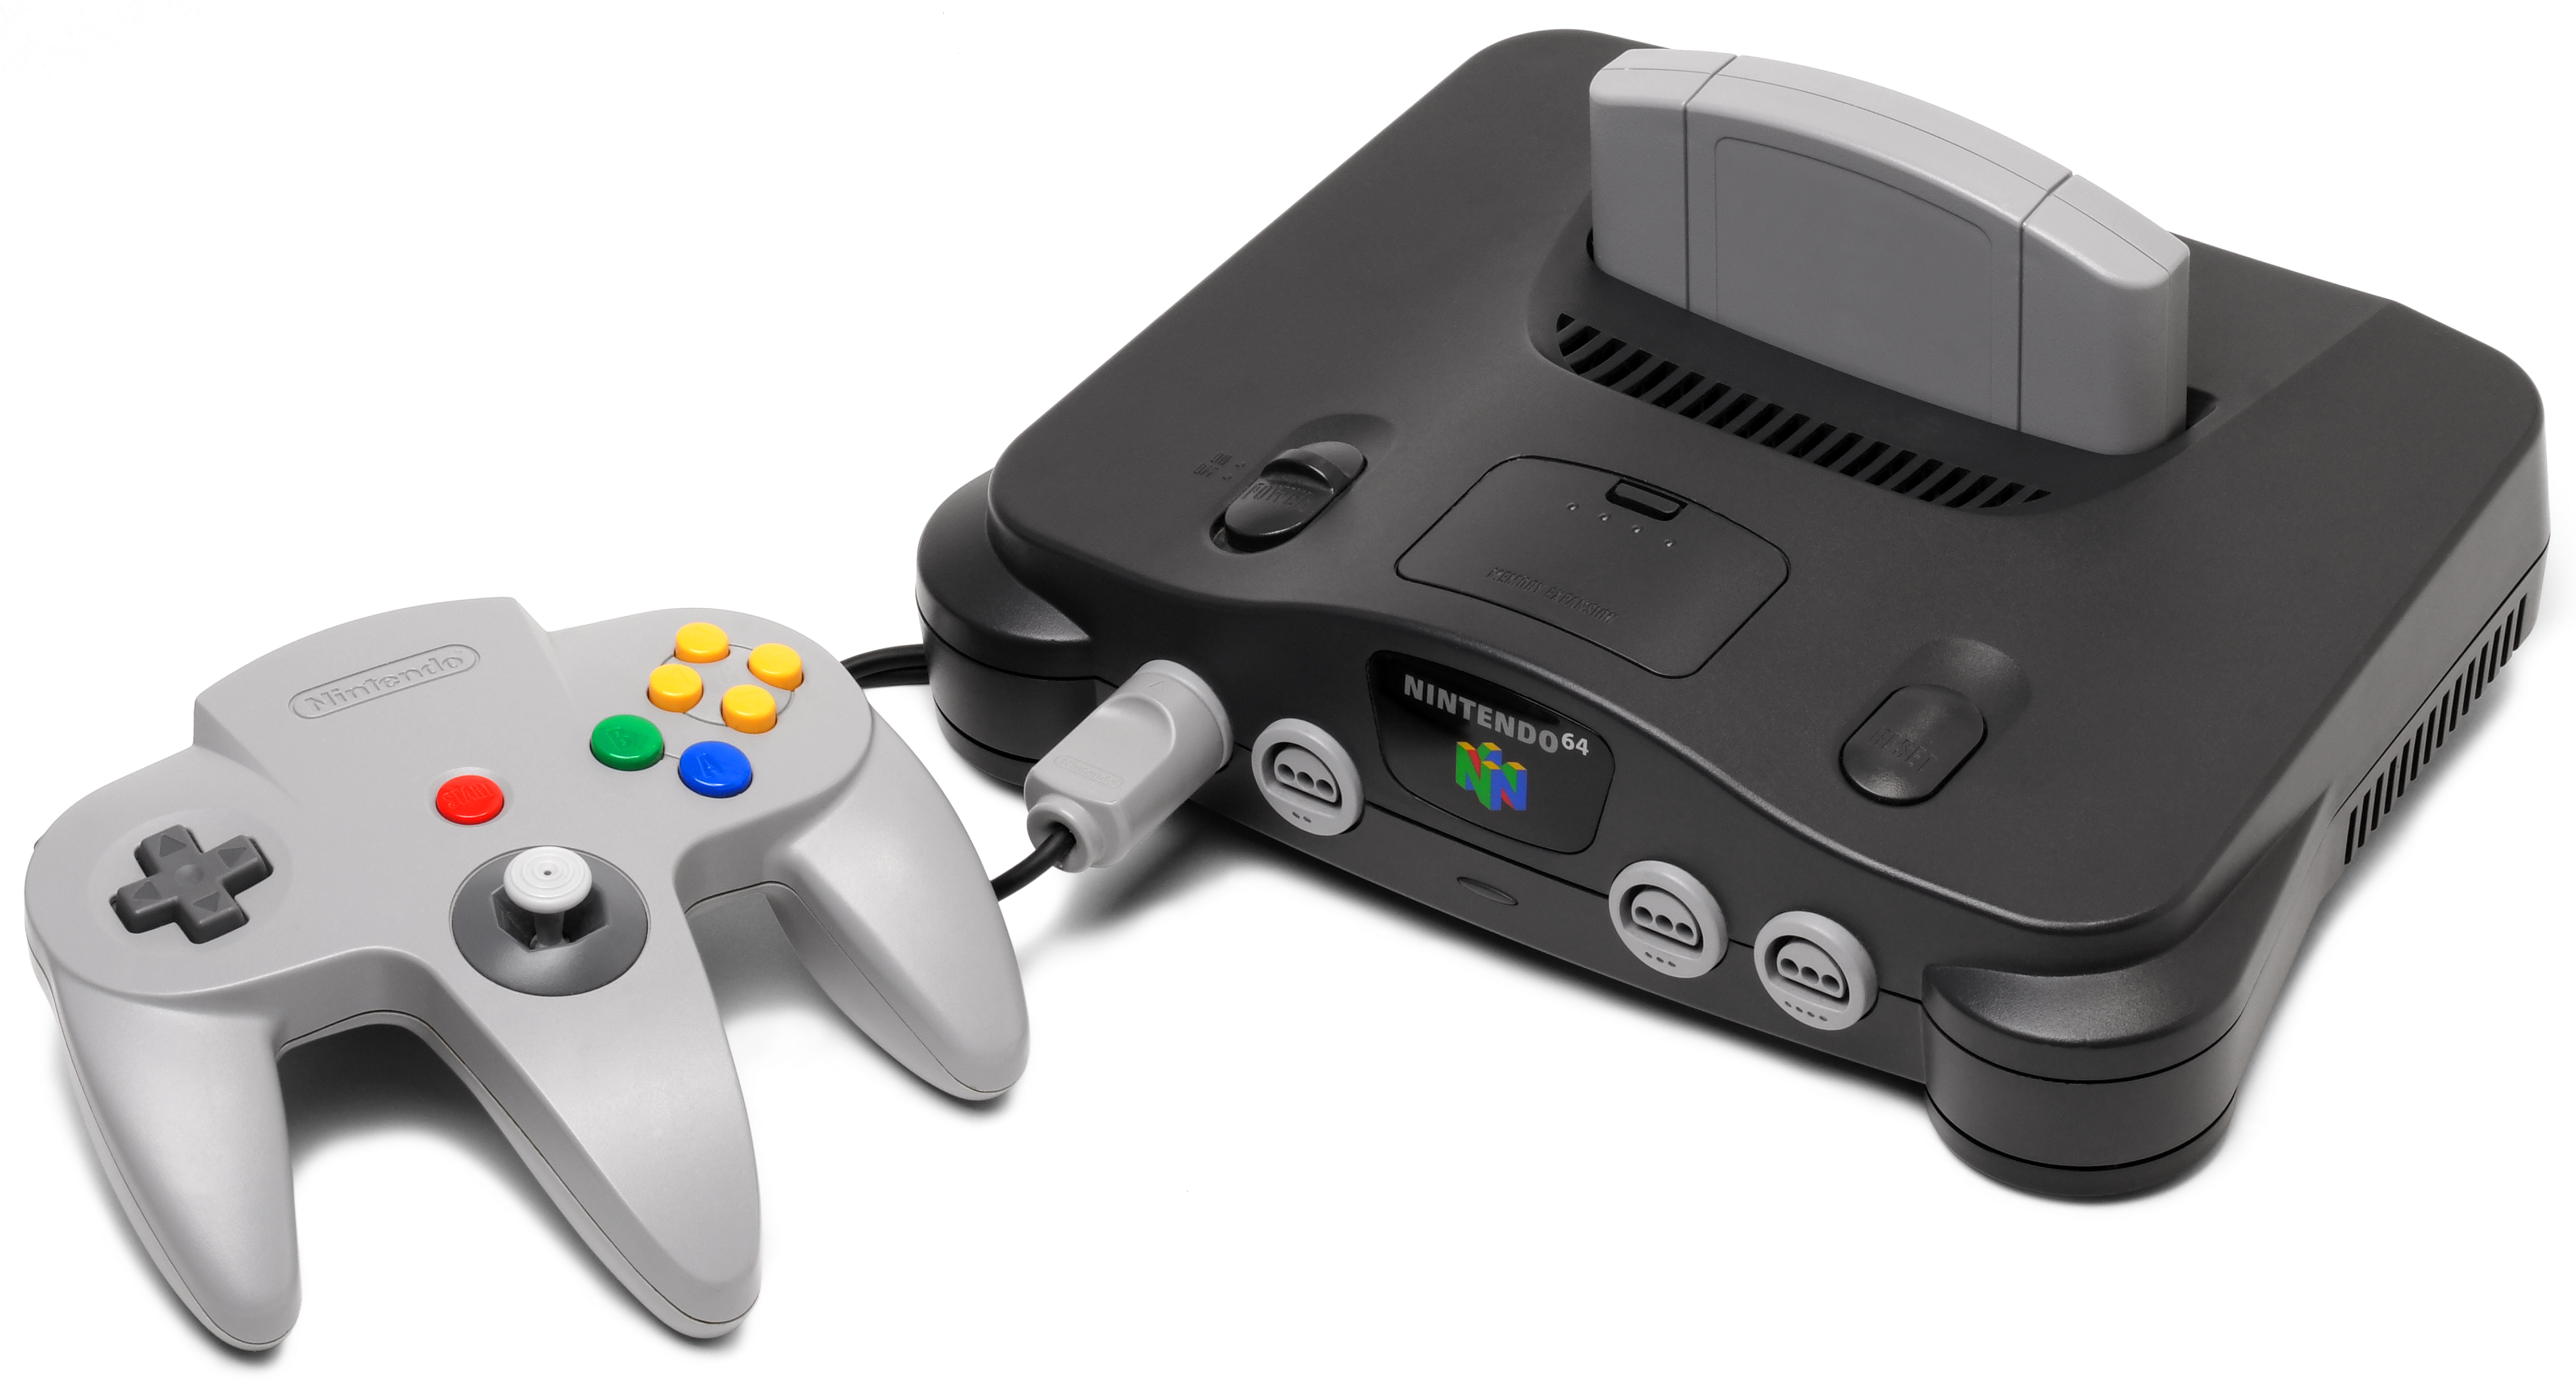
\includegraphics[width=0.4\textwidth]{./Imagenes/Bitmap/N64-Console-Set.png}
     }
     \hfill
 \subfloat[Rumble Pack Nintendo 64\label{quinta2}]{%
       \includegraphics[width=0.4\textwidth]{./Imagenes/Bitmap/rumble-pack-64.jpg}
     }
     \caption{Dispositivos de entrada relevantes en la 5"a  generaci\'on de consolas}
     \label{fig:quinta}
   \end{figure}


\subsection{Sexta generaci\'on (1998-2005)}

En los a\~nos posteriores las compa\~nias siguieron sacando diferentes mandos que modificaban tama\~no y posiciones de los botones pero no salieron cambios significativos hasta que en 2002 Nintendo lanz\'o al mercado un nuevo mando alternativo para su consola \textbf{GameCube}, este controlador ten\'ia la peculiaridad de ser inal\'ambrico. Lo llamaron \textbf{WaveBird Wireless Controller}[\ref{sexta1}] y sent\'o las bases para los pr\'oximos mandos inal\'ambricos. Contaba con una cruceta, 6 botones digitales, 2 botones h\'ibridos ya que hacian la funci\'on de gatillos y 2 palancas anal\'ogicas para el movimiento del personaje y la c\'amara normalmente. Como alimentaci\'on usaba 2 pilas AA y para comunicarse con la consola usaba radiofrecuencia, lo que permit\'ia al jugador alejarse hasta 6 metros de la consola. Poco tiempo despu\'es tanto Sony con su PlayStation 3 como Microsoft con su Xbox 360 a\~nadir\'ian las baterias a sus mandos para convertirlos en inal\'ambricos. \\


\begin{figure}[!ht]
     \subfloat[WaveBird Wireless Controller\label{sexta1}]{%
       \includegraphics[width=0.4\textwidth]{./Imagenes/Bitmap/Nintendo-GameCube-Wavebird-Silver.jpg}
     }
     \hfill
     \caption{Dispositivos de entrada relevantes en la 6"a  generaci\'on de consolas}
     \label{fig:sexta}
   \end{figure}

\subsection{Septa generaci\'on (2005-2012)}


\textbf{FALTA TODO LO DE WII QUE HAY QUE VOLVER A ESCRIBIR MEJOR.}

En 2010 Microsoft dio el salto a un nuevo controlador de videojuegos para su consola Xbox 360. Este nuevo perif\'erico es conocido con el nombre de \textbf{Kinect} y permite a los usuarios controlar e interactuar con la consola sin necesidad de tener contacto f\'isico con un mando tradicional. Este control se realiza por gestos y reconocimiento de voz. El sensor Kinect es una barra horizontal de unas 9 pulgadas conectada a una peque\~na base circular con un eje que permiteque esta rote y adem\'as est\'a dise\~nado para ser colocado por encima o por debajo de la televisi\'on. El dispositivo cuenta con una c\'amara RGB, un sensor de profundidad, un micr\'ofono de m\'ultiples matrices y un procesador personalizado que ejecuta el software patentado, que proporciona captura de movimiento de todo el cuerpo en 3D, reconocimiento facial y capacidades de reconocimiento de voz. El micr\'ofono de matrices del sensor de Kinect permite a la Xbox 360 llevar a cabo la localizaci\'on de la fuente ac\'ustica y la supresi\'on del ruido ambiente, permitiendo participar en el chat de Xbox Live sin utilizar auriculares. El sensor de profundidad es un proyector de infrarrojos combinado con un sensor CMOS monocromo que permite a Kinect ver la habitaci\'on en 3D en cualquier condici\'on de luz ambiental. El rango de detecci\'on de la profundidad del sensor es ajustable gracias al software de Kinect capaz de calibrar autom\'aticamente el sensor, basado en la jugabilidad y en el ambiente f\'isico del jugador, tal como la presencia de sof\'as, mesas y otro tipo de muebles.\\

PlayStation tambi\'en lanz\'o al mercado su dispositivo de control de videojuegos por movimiento, \textbf{PlayStation Move}, y es compatible con los sitemas PS3 y PS4. PlayStation Move compiti\'o tanto con el Kinect de Xbox como con el WiiMote de Nintendo. El dise\~no del mando consiste en un mando similar al de Wii ya que ambos se controlar con una mano en vertical. PlayStation Move uni\'o los conceptos de sensores de movimiento que usaba el WiiMote y la c\'amara que usaba el Kinect, por lo que PlayStation Move usa sensores de movimiento en el mando, una esfera en su extremo que se ilumina y la c\'amara PlayStation Eye que detecta la posici\'on del mando. Al igual que en el resto de controladores inal\'ambricos para PlayStation, tanto el mando principal de PlayStation Move como el Navigation Controller usan la conexi\'on inal\'ambrica Bluetooth 2.0 y una bater\'ia de ion de litio, que se carga mediante un puerto USB Mini-B. El Navigation Controller es un mando que complementa al mando principal y tiene una funci\'on similar a la del Nunchuck de Wii. Se pueden conectar hasta 4 PlayStation Move de manera simult\'anea.\\

\subsection{Octava generaci\'on (2012-2020)}

Coincidiendo con la salida al mercado del PlayStation Move, Nintendo lanz\'o su nueva consola en 2012; la \textbf{Wii U} y con ella un Controlador de videojuegos h\'ibrido. Este controlador h\'ibrido es el \textbf{Wii U GamePad} y es el mando principal de la consola. La principal distinci\'on con respecto a los mandos tradicionales es la incorporaci\'on de una pantalla t\'actil, la cual se utiliza para mostrar informaci\'on adicional durante una partida y adem\'as puede usarse como pantalla principal en caso de no disponer de un televisor mientras se juega. Adem\'as de como controlador de videojuegos, el Wii U GamePad es utilizado como control remoto independiente para cotrolar la pantalla de la televisi\'on u otro aparato via infrarrojos sin tener que tener la consola encendida. El mando constaba de altavoces y micr\'ofono e incorporaba una c\'amara frontal de 1.3 megapixeles. Los sensores que incorporaba eran: aceler\'ometro, giroscopio, geomagn\'etico e infrarrojo e incorporaba vibraci\'on. La conexi\'on a la consola se hac\'ia mediante bluetooth  y dispon\'ia de NFC para futuros accesorios que incorporaron a los diferentes videojuegos.\\

En 2013 Sony hizo una revisi\'on de su DualShock y como mando de la consola PlayStation 4 lanz\'o el \textbf{DualShock 4}. Este mando a\~nadi\'o al dise\~no anterior un panel t\'actil en la parte frontal, lo que hizo que la distribuci\'on de los botones que antes eran centrales cambiasen. En la parte trasera se a\~nadi\'o una barra LED que se ilumina en varios colores para diferenciar e identificar a los diferentes jugadores. Microsoft por su parte en 2015 puso a la venta su nuevo \textbf{Xbox One Elite Controller}. Una de las principales caracter\'isticas es que tiene un dise\~no modular por lo que cada pieza es intercambiable para que cada jugador pueda adaptarlo a su medida. La personalizaci\'on es el principal aliciente en este mando ya que permite reprogramar tanto los cuatro botones tradicionales de la parte frontal como los gatillos. Tambi\'en se da la posibilidad de establecer curvas de sensibilidad en las palancas anal\'ogicas. Gracias a la posibilidad de a\~nadir piezas, este mando incluye 4 palancas m\'as en la parte trasera.\\

En 2017 Nintendo present\'o su nueva consola h\'ibrida que se basa en su predecesora, Wii U. La consola es \textbf{Nintendo Switch} y es una consola que puede ser jugada tanto de manera port\'atil como de sobremesa en una televisi\'on o un monitor. Loa mando dise\~nados para esta consola son los \textbf{Joy Con} y consisten en 2 unidades, cada uno de ellos contiene una palanca anal\'ogica y una matriz de botones. Estos mandos tienen la peculiaridad de que pueden usarse tanto acoplados a la consola cuando esta se utilice en modo port\'atil o pueden ser desacoplados para cuando la consola se utilice en una televisi\'on. Cuando se separan, un par de Joy-Con pueden ser utilizados por un solo jugador, o dividido entre dos como controladores individuales. Los Joy-Con se distribuyen en pares, designados como ``Joy-Con L'' y ``Joy-Con R'', respectivamente. Una misma Nintendo Switch puede tener conectados hasta un total de 8 Joy-Con. La comunicaci\'on que tienen con la consola se realiza por Bluetooth. Los Joy-Con contienen bater\'ias no extraibles de 525 mAh, que se cargan cada vez que se conectan a la consola. Ambos controladores contienen una palanca anal\'ogica, cuatro botones de cara, dos botones superiores, dos botones laterales accesibles cuando se sueltan y designados como SL y SR, un bot\'on ``+'' o ``-'', un bot\'on de sincronizaci\'on y un indicador de jugador luces LED. Cada uno de los Joy-Con contiene un aceler\'ometro y un giroscopio, que pueden ser utilizados para los juegos que incluyen movimiento. Adem\'as, el Joy-Con R contiene un sensor de seguimiento de profundidad infrarroja, que puede leer objetos y movimientos sostenidos delante de \'el. Cada uno de los Joy-Con incorpora un motor para la vibraci\'on del mando durante las sesiones de juego.\\

Tambi\'en durante 2017, Sony anunci\'o una serie de juegos nuevos que se jugar\'ian de una forma totalmente diferente ya que el mando utilizado ser\'ia cada uno de los tel\'efonos m\'oviles de los usuarios. A esta serie de juegos se la conoce como \textbf{PlayLink}. La idea detr\'as de PlayLink es que todos los usuarios de la consola PlayStation 4 y sus familiares y amigos disponen de un dispositivo m\'ovil pero no todos disponen de varios mandos para poder jugar con m\'as personas en juegos cooperativos. PlayLink es una aplicaci\'on m\'ovil que cada usuario se descarga en su Android o iOS y as\'i puede usar su tel\'efono como un mando m\'as de PlayStation 4. El requisito para que la conexi\'on sea efectiva es que tanto la consola PS4 como los dispositivos m\'oviles que se vayan a usar est\'en conectados a la misma red WIFI.\\

\subsection{Novena generaci\'on (2020-Actual)}

A finales del a\~no 2020 Sony lanz\'o al mercado su nueva consola, la PS5 y con ella un nuevo mando al que bautizaron como \textbf{DualSense}. Como ya pasaba con el DualShock 4, este mando funciona con bater\'ia y lleva un altavoz integrado. La gran novedad que trae este mando es la retroalimentaci\'on h\'aptica. Se han sustituido los motores de vibraci\'on tradicionales por 2 activadores que emiten vibraciones din\'amicas capaces de simular todo tipo de sensaciones. Adem\'as de la nueva retroalimentaci\'on h\'aptica, el nuevo DualSense incorpora 2 gatillos adaptativos. Estos gatillos emiten diferente fuerza de resistencia contra el jugador dependiendo del arma que se est\'e utilizando. El ejemplo que pusieron los desarrolladores de Sony fue con la cuerda de un arco, inicialmente no tiene resistencia pero cuanto m\'as se tense la cuerda del arco m\'as fuerza es necesaria.

\section{\textit{Feedback} en los controladores}

En los inicios de los videojuegos y de las consolas el objetivo fue la creaci\'on de nuevos tipos de juegos con diferentes mec\'anicas y mejoras gr\'aficas. En la era actual de los videojuegos se ha ido mucho m\'as lejos de los primeros juegos como Pong y Tetris, la tendencia ha llevado a la creaci\'on de escenarios virtuales m\'as realistas y a que el jugador formase parte de ese entorno virtual. Particularmente la respuesta que se da al usuario del videojuego al realizar acciones es conocida como \textbf{tecnolog\'ia h\'aptica}. Este tipo de tecnolog\'ia se refiere al conjunto de interfaces tecnol\'ogicos que interaccionan con una persona mediante el sentido del tacto. La tecnolog\'ia h\'aptica tiene sus inicios en los dispositivos de los sistemas servo para controlar grandes aviones con la intenci\'on de poder hacerlo de manera remota. En estos sistemas se instal\'o un sistema de control que proporcionaba una resistencia a la palanca del piloto proporcional al \'angulo de ataque del avi\'on. Otro ejemplo destacable de esta tecnolog\'ia se encuentra en la pel\'icula \textbf{4-D Honey, I Shrunk the Audience!} del a\~no 1994 que simulaba que los ratones se soltaban por el auditorio y corrian por toda la sala. Para conseguir esta simulaci\'on se bombeaba aire a trav\'es de un peque\~no tubo de pl\'astico y al agitarse, imitaba la sensaci\'on de las colas de los ratones rozando las piernas de los espectadores. \\

En los videojuegos esta tecnolog\'ia fue introducida a trav\'es de los controladores. Al inicio estos sistemas de vibraci\'on se introdujeron en los controladores como dispositivos que se acoplaban al mando por separado como pasaba con el \textbf{Rumble Pack} de Nintendo 64. Con la salida del \textbf{Dualshock} en su versi\'on japonesa esto cambi\'o. Este mando incorporaba un sistema de vibraci\'on conocido como \textit{tabletas vibradoras (rumble packs)} que ten\'ian ese efecto de vibraci\'on al conducir veh\'iculos o disparar armas de fuego. Con la llegada de las pantallas t\'actiles tambi\'en aparecieron las pantallas h\'apticas. Estas pantallas son aquellas que transmiten una vibraci\'on al tocarla. El ejemplo m\'as actual de tecnolog\'ia h\'aptica puede encontrarse en la reciente consola de Nintendo, Nintendo Switch. Nintendo no ha denominado a la tecnolog\'ia que usan sus Joy-Cons como tecnolog\'ia h\'aptica sino como \textbf{Rumble HD}. 


\section{Sistemas de \textit{streaming} en videojuegos}

Con la extensi\'on de los dispositivos m\'oviles en el mundo de los videojuegos y las mejoras en las conexiones a internet, la industria de los videojuegos se mueve a pasos acelerados hacia el \textit{gaming} en la nube. Servicios de retransmisi\'on via streaming como \textit{Netflix} o \textit{Amazon Prime Video} ofrecen la posibilidad de disponer de un cat\'alogo de series a peliculas a trav\'es de internet. Con este precedente, empresas como Google\footnote{https://stadia.google.com/} y Nvidia\footnote{https://www.nvidia.com/es-es/geforce-now/} se han adentrado al mundo de los juegos en la nube.\\

Esta nueva forma de forma no solamente consiste en retransmitir al usuario final ala partida que est\'a jugando sino que el proceso va mucho m\'as all\'a. Esta diferencia tiene lugar a la hora de tratar el input del usuario. En un videojuego tradicional, ejecutado en la misma m\'aquina en la que se est\'a jugando, una vez el usuario realiza una entrada el videojuego lo procesa y genera una respuesta apropiada. En los videojuegos en la nube una vez el usario realiza una acci\'on, esta debe ser enviada al servidor donde el juego est\'a siendo ejecutado. Una vez en el servidor, la entrada que gener\'o el usuario es tratada y se realizan los cambios en el estado del juego que haya probocado el usuario con su entrada. Cuando el estado cambia en el servidor se prepara el frame, se codifica y es enviado de vuelta al usuario que tendr\'a que decodificar el frame una vez le llegue al dispositivo donde est\'e jugando \citep{cloudgaming}.

Los anchos de banda requeridos para estas dos tecnolog\'ias var\'ian con las resoluciones a las que se quiera jugar [\ref{stadiovsgeforce}]. Ambos sistemas aconsejan una conexi\'on Ethernet o un router que disponga de una red de frecuencia 5 GHz.

\begin{table}[h]
    \centering
    \begin{tabular}{lll}
        \toprule
        {}  & \textbf{Google Stadia} & \textbf{Nvidia GeForce Now} \\
        \midrule
        \textbf{720p 60fps} & 10 Mbps & 15 Mbps\\
        \textbf{1080p 60fps} & 20 Mbps & 25 Mbps \\
		\textbf{4K 60fps} & 35Mbps & No Disponible \\
        \bottomrule
    \end{tabular}
\caption{Ancho de banda necesario para jugar a Stadia vs GeForce Now}
\label{stadiovsgeforce}
\end{table}


%-------------------------------------------------------------------


% Variable local para emacs, para  que encuentre el fichero maestro de
% compilaci�n y funcionen mejor algunas teclas r�pidas de AucTeX
%%%
%%% Local Variables:
%%% mode: latex
%%% TeX-master: "../ManualTeXiS.tex"
%%% End:




\begin{FraseCelebre}
\begin{Frase}
%Si quieres ser le�do m�s de una vez, no vaciles en borrar a menudo.
%Rem tene, verba sequentur (Si dominas el tema, las palabras vendr�n solas)
\end{Frase}
\begin{Fuente}
%Horacio
%Cat�n el Viejo
\end{Fuente}
\end{FraseCelebre}


\chapter{Especificaci\'on del protocolo de comunicaci\'on}
\label{cap3}
\label{cap:especificacion}


La finalidad de este trabajo es conseguir la conexi\'on entre 2 dispositivos con la creaci\'on de una librer\'ia para un motor de videojuegos. Uno de ellos va funcionar como un controlador de videojuegos y otro como ejecutor del juego. Para que esta comunicaci\'on se consiga es necesario analizar y definir las funcionalidades que se quieren ofrecer a los desarrolladores que usen la librer\'ia. \\

En este cap\'itulo se va realizar un an\'alisis de las diferentes funcionalidades que son necesarias para que la comunicaci\'on pueda realizarse. Se expondr\'an las ventajas y las desventajas de cada una de estas funcionalidades y por \'ultimo se definir\'a el protocolo de comunicaci\'on entre los 2 dispositivos involucrados en este trabajo.


%-------------------------------------------------------------------
\section{Arquitectura del proyecto a alto nivel}
%-------------------------------------------------------------------

\begin{figure}[!htb]
    \centering
    \includegraphics[width=0.90\textwidth]{./Imagenes/Vectorial/Diagrama protocolo.pdf}
    \caption{Esquema de comunicaci\'on del proyecto}
\label{Fig:arquitectura}
\end{figure}

Como ya hemos mencionado, el objetivo a alto nivel se explica en la figura~\ref{Fig:arquitectura}. 

Para conseguir usar el dispositivo m\'ovil como mando para videojuegos se plantearon las posibles caracter\'isticas que podr\'ian incluirse. Como se detalla m\'as adelante, estas opciones difieren en la versatilidad que se le ofrece al usuario de la librer\'ia, la complejidad de programaci\'on y el ancho de banda usado durante la ejecuci\'on del juego. \\

La primera de estas opciones se basa en el uso de im\'agenes est\'aticas de mandos cargados previamente en la aplicaci\'on del m\'ovil. La comunicaci\'on entonces ser\'ian las pulsaciones que se env\'ian desde el m\'ovil al ordenador.  En este esquema el feedback viene dado por la aplicaci\'on que se ejecuta en el dispositivo m\'ovil. La principal ventaja en el env\'io de una \'unica imagen est\'atica es el poco uso de ancho de banda. La \'unica comunicaci\'on que se tiene por red es el env\'io de las pulsaciones del usuario en la pantalla del m\'ovil al ordenador. Esta comunicaci\'on puede realizarse utilizando TCP y conseguir as\'i que no se pierda ninguna pulsaci\'on del usuario. Otra ventaja que ofrece es la poca complejidad que supone para el usuario final de la librer\'ia. Con este sistema, el juego ser\'ia notificado de la llegada de pulsaciones desde el tel\'efono gracias a la librer\'ia desarrollada. El desarrollador del juego \'unicamente tendr\'ia que encargarse de decidir qu\'e hacer con la llegada de cada pulsaci\'on. Esto lleva directamente a la primera desventaja, la poca versatilidad que se le da al usuario de la librer\'ia. Al no haber una comunicaci\'on desde el videojuego hasta el m\'ovil, perdemos la oportunidad de que el desarrollador del juego modifique el mando que quiere utilizar o que ordene al tel\'efono activar la vibraci\'on a su gusto.\\

Para resolver el problema de la modificaci\'on del mando que usar se plante\'o una nueva caracter\'istica: permitir que el juego env\'ie im\'agenes en formato .PNG a lo largo de la sesi\'on de juego. Para que esto sea posible se tiene que habilitar el env\'io de datos en ambas direcciones. Hacer esto supone un aumento en el uso necesario del ancho de banda a cambio de dar m\'as versatilidad al usuario de la librer\'ia. Para conseguir la modificaci\'on de las im\'agenes, Android ofrece un sistema de capas en las im\'agenes que se describan en el archivo de manifiesto. Estas capas se pintan en orden descendiente, siendo la \'ultima im\'agen declarada la que tapar\'ia al resto. \\

Para disminuir el impacto en el ancho de banda se plante\'o la opci\'on de que el env\'io del mando desde el juego al dispositivo m\'ovil se hiciese \'unicamente al inicio de la conexi\'on. Hacerlo de esta manera permitir\'ia al usuario de la librer\'ia modificar el mando con el que se quiere jugar pero este no se podr\'ia cambiar en ning\'un momento de la ejecuci\'on. Esta decisi\'on aumenta el coste en el ancho de banda al inicio de la conexi\'on pero disminuye dr\'asticamente una vez que la imagen del mando ha sido guardada, lo que permite seguir usando TCP como protocolo de transmisi\'on.\\


Otra nueva caracter\'istica da la posibilidad al usuario de la librer\'ia de enviar streaming de video al dispositivo m\'ovil y que este lo muestre por pantalla. Para que esto sea posible la comunicaci\'on entre ambos dispositivos tiene que realizarse en ambos sentidos durante toda la ejecuci\'on con un intercambio constante de datos. Como esta caracter\'isitica es la m\'as vers\'atil para el usuario de la librer\'ia, en esta arquitectura se dar\'ia la posibilidad de controlar la vibraci\'on tambi\'en al desarrollador. Darle todas estas caracter\'isticas al desarrollador implica un aumento en la complejidad del c\'odigo que este tiene que implementar. Dado que el consumo del ancho de banda sube de manera considerable, en este dise\~no se ha optado por modificar el protocolo de transmisi\'on de TCP a UDP para disminuir el consumo. Esta caracter\'istica es m\'as vers\'atil para el desarrollador del videojuego pero tambi\'en es m\'as costosa en cuanto al ancho de banda que usa. Esto implica que se asume una posible p\'erdida de pulsaciones realizadas por el usuario o una posible p\'erdida de frames en el env\'io del streaming de video.\\

Este \'ultimo conjunto de caracter\'isticas ha sido el utilizado para este proyecto. Las funcionalidades que se ofrecen al usuario de la librer\'ia son:

\begin {itemize}
\item Env\'io de pulsaciones desde el dispositivo m\'ovil al juego.
\item Env\'io de streaming de im\'agenes en formato .PNG desde el juego al m\'ovil.
\item Env\'io de orden de vibraci\'on del juego al m\'ovil.
\end {itemize}

Para que el desarrollador tenga un control total de lo que se env\'ia en cada momento, se da la opci\'on de enviar un mensaje de vibraci\'on al dispositivo m\'ovil. Esto permite que el m\'ovil vibre no solo por las pulsaciones, sino, por ejemplo, cuando el jugador reciba da\~no o se choque si est\'a jugando a un juego de conducci\'on. En la siguiente secci\'on se detalla el protocolo desarrollado y en el pr\'oximo cap\'itulo se detallar\'a la implementaci\'on de la parte de m\'ovil y PC.


%-------------------------------------------------------------------
\section{Protocolo de comunicaci\'on entre juego y dispositivo de entrada}
%-------------------------------------------------------------------

Un protocolo de comunicaci\'on es un sistema de reglas que permiten a 2 o m\'as dispositivos comunicarse entre ellos. Estas reglas se establecen para permitir la transmisi\'on de datos y la forma en la que la informaci\'on debe ser procesada. Cada mensaje tiene un significado exacto destinado a obtener una respuesta de un rango de posibles respuestas predeterminadas para esa situaci\'on en particular. Una de las caracter\'isticas principales de un protocolo de comunicaci\'on es que ambas partes tienen que conocer y usar los mensajes que se van a enviar y a recibir. \\

La estructura de estos mensajes consta de 2 partes: el primer byte define el tipo del mensaje y en los bytes posteriores viene la informaci\'on esperada. Con esto se consigue tener un tama\~no de datagrama diferente dependiendo de la informaci\'on que requiera mensaje. Adem\'as, es ampliable en caso de querer definir mensajes nuevos ya que no se utilizan todos los valores de este primer byte. En los siguientes p\'arrafos se van a describir cada uno de los mensajes que est\'an definidos para este protocolo. \\

El byte de cabecera indica el tipo de mensaje y la informaci\'on que se espera. En esta primera versi\'on del protocolo se han utilizado los 7 primeros valores. Existen 2 mensajes que no tienen cabecera, el primer mensaje que realiza la conexi\'on y el env\'io de la resoluci\'on del dispositivo m\'ovil. Para que la conexi\'on se realice con \'exito, el dispositivo de entrada debe enviar la versi\'on del protocolo en la que se encuentra. En caso de que la versi\'on coincida en ambos dispositivos, la conexi\'on se dar\'a por buena. Tras el env\'io de la versi\'on del protocolo, el dispositivo m\'ovil enviar\'a su resoluci\'on para (tabla~\ref{table:1}). En caso contrario, el mensaje es descartado ya que contestar a este mensaje puede ser una brecha de seguridad. Al utilizar UDP, contestar a mensajes de conexi\'on fallidos puede desembocar en un ataque similar a una inundaci\'on UDP, \cite{udpflood}.\\


\begin{table}[h!]
\centering
\begin{tabular}{|c|c|} 
\hline
0-15                   & 16-32                   \\
\hline
 \multicolumn{1}{|c|}{Ancho} & \multicolumn{1}{c|}{Alto}  \\
\hline
\end{tabular}
\caption{Env\'io de la resoluci\'on del m\'ovil al juego.}
\label{table:1}
\end{table}

Una vez los 2 primeros mensajes son enviados, los siguientes se enviar\'an de forma as\'incrona y se diferencian por el primer byte del datagrama. Este primer byte tiene como funci\'on ser usado como cabecera y poder diferenciar cada tipo de mensaje. Los posibles mensajes son:\\

\begin {itemize}
\item El valor de cabecera 0 es utilizado para los mensajes de tipo pulsacion. Estos mensajes son enviados desde el dispositivo m\'ovil (tabla~\ref{table:2}).
\item  El valor de cabecera 1 es utilizado para los mensajes de tipo \textit{tracker}. 
\item  El valor de cabecera 2 es utilizado para avisar al dispositivo m\'ovil de activar la vibraci\'on durante un tiempo establecido.
\item  El valor de cabecera 3 es utilizado para enviar im\'agenes comprimidas desde el juego al m\'ovil.
\item  El valor de cabecera 4 es utilizado para avisar sobre el cierre de conexi\'on por parte del dispositivo que lo env\'ia.
\item  El valor de cabecera 5 es utilizado para establecer el tiempo de vibraci\'on en caso de que este se active (tabla~\ref{table:3}).
\item  El valor de cabecera 6 es utilizado para los mensajes \textit{keep alive}, utilizados para comprobar que la conexi\'on sigue activa en caso de que el usuario no realice pulsaciones en un tiempo determinado.
\end {itemize}

%----------------------------------------------------------------------------------------------------------

\begin{table}[h!]
\centering
\begin{tabular}{|c|c|c|c|} 
\hline
Byte de cabecera                   & 8-15                            & 16-31 & 32-47 \\ 
\hline
\multicolumn{1}{|c|}{00000000} & Tipo de pulsaci\'on & \multicolumn{1}{c|}{Posici\'on X} & \multicolumn{1}{c|}{Posici\'on Y}  \\
\hline
\end{tabular}
\caption{Pulsaci\'on enviada desde el dispositivo m\'ovil al ejecutor del juego}
\label{table:2}
\end{table}

%----------------------------------------------------------------------------------------------------------

\begin{table}[h!]
\centering
\begin{tabular}{|c|c|} 
\hline
Byte de cabecera                                     & 8-23                   \\
\hline
\multicolumn{1}{|c|}{00000101} & \multicolumn{1}{c|}{Tiempo de vibraci\'on}  \\
\hline
\end{tabular}
\caption{Tiempo de vibraci\'on del dispositivo m\'ovil en milisegundos}
\label{table:3}
\end{table}

%----------------------------------------------------------------------------------------------------------

Los mensajes de los que no se ha puesto ninguna tabla es porque son utilizados para avisar de eventos, por lo que con la cabecera es suficiente. El tiempo de vibraci\'on del dispositivo puede modificarse en cualquier momento para que el usuario de la librer\'ia pueda modificarla en funci\'on del momento del juego. En la figura~\ref{Fig:protocolo} se puede observar el flujo de datagramas durante una ejecuci\'on del juego.\\

\begin{figure}[h]

\centering
\includegraphics[width=0.7\textwidth]{./Imagenes/Vectorial/Arquitectura}
\caption{Diagrama del protocolo de comunicaci\'on entre ambos dispositivos}
\label{Fig:protocolo}
\end{figure}

Las im\'agenes enviadas est\'an comprimidas en formato PNG (\cite*{pngdefinitiveedition}). El tama\~no de esta im\'agen puede variar en funci\'on de la complejidad de la im\'agen. En pruebas realizadas, esta im\'agen pesa aproximadamente 24KB, un valor bastante inferior a los 64KB que admite UDP como tama\~no m\'aximo de paquete (\cite*{udp}). En este protocolo no se ha tenido en cuenta la divisi\'on de datagramas por superar el tama\~no m\'aximo soportado por UDP.\\

\vspace{30mm}

\bigskip
\Large{\textbf{En el pr\'oximo cap\'itulo}}\\
\normalsize

Tal y como hemos visto en este cap\'itulo, para la realizaci\'on de este proyecto surgieron 3 alternativas de las posibles caracter\'isticas que deber\'ia incorporar. Tras analizar las ventajas y desventajas se escogi\'o la que mayor versatilidad daba al desarrollador a cambio de un mayor coste en el ancho de banda. Para solventar esto se decidi\'o utilizar UDP como protocolo de transmisi\'on. En el pr\'oximo cap\'itulo se procede a explicar la implementaci\'on tanto de la aplicaci\'on de Android como de  la aplicaci\'on de Unity. 


% Variable local para emacs, para  que encuentre el fichero maestro de
% compilaci�n y funcionen mejor algunas teclas r�pidas de AucTeX
%%%
%%% Local Variables:
%%% mode: latex
%%% TeX-master: "../ManualTeXiS.tex"
%%% End:

%\include{Capitulos/Parte2}
%---------------------------------------------------------------------
%
%                          Cap�tulo 4
%
%---------------------------------------------------------------------
%
% 04Imagenes.tex
% Copyright 2009 Marco Antonio Gomez-Martin, Pedro Pablo Gomez-Martin
%
% This file belongs to the TeXiS manual, a LaTeX template for writting
% Thesis and other documents. The complete last TeXiS package can
% be obtained from http://gaia.fdi.ucm.es/projects/texis/
%
% Although the TeXiS template itself is distributed under the 
% conditions of the LaTeX Project Public License
% (http://www.latex-project.org/lppl.txt), the manual content
% uses the CC-BY-SA license that stays that you are free:
%
%    - to share & to copy, distribute and transmit the work
%    - to remix and to adapt the work
%
% under the following conditions:
%
%    - Attribution: you must attribute the work in the manner
%      specified by the author or licensor (but not in any way that
%      suggests that they endorse you or your use of the work).
%    - Share Alike: if you alter, transform, or build upon this
%      work, you may distribute the resulting work only under the
%      same, similar or a compatible license.
%
% The complete license is available in
% http://creativecommons.org/licenses/by-sa/3.0/legalcode
%
%---------------------------------------------------------------------

\chapter{Implementaci\'on de las aplicaciones}
\label{cap4}
\label{cap:impl}

En este cap\'itulo se detalla todo el proceso de creaci\'on y desarrollo de las diferentes aplicaciones y la demo que posteriormente se utiliza como ejemplo de implementaci\'on de la herramienta.
Se ha divido este cap\'itulo en 3 secciones:

\begin {itemize}
\item Implementaci\'on de la aplicaci\'on de Android.
\item Implementaci\'on de la aplicaci\'on de Unity.
\item Inclusi\'on de la herramienta en un juego cerrado.
\end {itemize}

%-------------------------------------------------------------------
\section{Implementaci\'on de la aplicaci\'on de Android}
%-------------------------------------------------------------------

Este proyecto se ha desarrollado utilizando principalmente 2 tecnolog\'ias: el motor de Unity y Android. Al tratarse de un proyecto de creaci\'on de un controlador para videojuegos y tomando como base la especificaci\'on desarrollada en el cap\'itulo 3 se ha optado por el desarrollo de una aplicaci\'on para Android que sirva como dispositivo de entrada y una aplicaci\'on en Unity que sirva como ejecutor del juego.

Android Studio es el entorno de desarrollo integrado (IDE) oficial para la plataforma de Android. Hasta finales del 2014 para desarrollar en Android se utilizaba Eclipse como IDE oficial y est\'a disponible para las plataformas Microsoft Windows, macOS y GNU/Linux. Android Studio incluye una gran variedad de herramientas para facilitar el desarrollo en Android entre las que se incluyen:

\begin {itemize}
\item Plantillas para crear dise\~nos comunes de Android y otros componentes.
\item Un editor de dise\~no enriquecido que permite a los usuarios arrastrar y soltar componentes de la interfaz de usuario.
\item Soporte para construcci\'on basada en Gradle.
\item Un dispositivo virtual de Android que se utiliza para ejecutar y probar aplicaciones.
\item Consola de desarrollador: consejos de optimizaci\'on, ayuda para la traducci\'on y estad\'isticas de uso.
\item Integraci\'on de ProGuard y funciones de firma de aplicaciones.
\end {itemize}
 
Los lenguajes de programaci\'on aceptados por Android Studio son Kotlin, Java y C++. En concreto para este proyecto se ha usado Java como lenguaje de programaci\'on.

%-------------------------------------------------------------------
\subsection {Ciclo de vida de Android}
%-------------------------------------------------------------------

Las aplicaciones en Android se rigen por una serie de componentes que se llaman \textbf{\textit{Activity}}. Estos componentes son claves a la hora de manejar los estados de una aplicaci\'on en Android. A diferencia de otros paradigmas de programaci\'on que comienzan sus aplicaciones con un m\'etodo \textbf{\textit{main()}}, la instancia de una Actividad invoca m\'etodos de devoluci\'on de llamada que se corresponden con etapas espec\'ificas de su ciclo de vida. La experiencia de una aplicaci\'on para un dispositivo m\'ovil difiere mucho de la versi\'on de escritorio de esa misma aplicaci\'on ya que la interacci\'on del usuario con la aplicaci\'on no siempre comienza en el mismo lugar. Un claro ejemplo de esto sucede con las aplicaciones de mensajer\'ia instantanea. Un usuario puede estar navegando por cualquier red social y encontrarse una publicaci\'on interesante y compartirla por correo electr\'onico o por una aplicaci\'on de mensajer\'ia instantanea. La aplicaci\'on de correo electr\'onico no se abre en el mismo estado si se abre desde la opci\'on de compartir de la red social o si se abre desde el men\'u de aplicaciones instaladas en el dispositivo. Las Actividades est\'an dise\~nadas para facilitar este paradigma.

La mayor\'ia de las aplicaciones contienen varias pantallas, lo cual significa que contienen varias actividades. Este concepto se pondr\'a posteriormente de manifiesto ya que para el desarrollo de la aplicaci\'on han sido necesarias 2 Actividades. Una actividad proporciona una ventana en la que la aplicaci\'on dibuja la interfaz de usuario. Esta ventana puede estar a pantalla completa o puede ser m\'as peque\~na y flotar sobre otras ventanas como si fuese un \textit{pop-up}.

Cuando un usuario navega por una aplicaci\'on, la cierra, la vuelve a abrir o la minimiza, las instancias de las Actividades de la aplicaci\'on pasan por una serie de estados de su ciclo de vida. Estos estados pueden tener comportamientos definidos por los desarrolladores de la aplicaci\'on. Esto permite tener un control sobre lo que ocurre en cada uno de los estados de la aplicaci\'on. Para navegar por las transiciones entre las etapas del ciclo de vida de una actividad, la clase Activity proporciona un conjunto b\'asico de seis devoluciones de llamadas: \textbf{onCreate() ,onStart(), onResume(), onPause(), onStop() y onDestroy().} El sistema invoca cada una de estas devoluciones de llamada cuando una operaci\'on entra en un nuevo estado.


\begin{figure}[h]

\centering
\includegraphics[width=0.7\textwidth]{./Imagenes/Bitmap/Ciclo_de_vida_Android}
\caption{Ciclo de vida de una Actividad de un sistema Android}
\end{figure}


Cada uno de los estados que tiene la actividad es llamado en un momento concreto de la ejecuci\'on de la Actividad. Las caracter\'isticas de cada uno de estos estados son las siguientes:

\begin {itemize}
\item \textbf{onCreate()} $\rightarrow$ Este m\'etodo es el primero que llama cuando se crea la Actividad. Este estado es utilizado para ejecutar la l\'ogica de la aplicaci\'on que debe ocurrir \'unicamente una vez en todo el ciclo de vida. Este m\'etodo recibe el par\'ametro \textit{\textbf{savedInstanceState}}, que es un objeto de tipo \textbf{\textit{Bundle}} que contiene el estado ya guardado de la actividad. Si la actividad nunca existi\'o, el valor del objeto \textit{Bundle} es nulo.
\item \textbf{onStart()} $\rightarrow$ Cuando la actividad entra en el estado Started, el sistema invoca esta devoluci\'on de llamada. La llamada \textit{onStart()} hace que el usuario pueda ver la actividad mientras la app se prepara para que esta entre en primer plano y se convierta en interactiva. Por ejemplo, este m\'etodo es donde la app inicializa el c\'odigo que mantiene la IU.
\item \textbf{onResume()} $\rightarrow$  La aplicaci\'on permanece en este estado hasta que ocurre alg\'un evento que la quita de foco. Tal evento podr\'ia ser, por ejemplo, recibir una llamada telef\'onica, que el usuario navegue a otra actividad o que se apague la pantalla del dispositivo.
\item \textbf{onPause()} $\rightarrow$ Este estado se utiliza cuando se ha perdido el foco de una aplicaci\'on. Sin embargo una actividad con el estado Paused puede ser completamente visible si est\'a en el modo multiventana. En este estado no deben guardarse datos de la aplicaci\'on ya que es un estado que dura poco tiempo.
\item \textbf{onStop()} $\rightarrow$ En este estado es donde los componentes del ciclo de vida pueden detener cualquier funcionalidad que no necesite ejecutarse mientras el componente no sea visible en la pantalla. Este estado debe usarse para liberar o ajustar recursos que no son necesarios mientras no sea visible para el usuario.
\item \textbf{onDestroy()} $\rightarrow$ Se llama a este m\'etodo antes de que se finalice la actividad. El sistema invoca esta devoluci\'on de llamada cuando el dispositivo rota o cuando la aplicaci\'on se cierra. En este estado es donde los componentes del ciclo de vida pueden recuperar cualquier elemento que se necesite antes de que finalice la Actividad.
\end {itemize}

%-------------------------------------------------------------------
\subsection {Arquitectura de la aplicaci\'on Android}
%-------------------------------------------------------------------

Para que la aplicaci\'on Android cumpla los requisitos expuestos en el apartado de especificaci\'on del proyecto, se han implementado 3 clases:

\begin {itemize}
\item \textbf{Controller} $\rightarrow$ Esta es la actividad principal. Desde esta actividad se recogen los datos de IP y puerto al que debe conectarse el dispositivo Android para ser utilizado como controlador.Al crearse la Actividad se lanza la ejecuci\'on de una hebra que se encargar\'a de recibir, leer e interpretar las im\'agenes que lleguen por red una vez la aplicaci\'on se conecte al juego. Desde esta clase se controla la pulsaci\'on del usuario en la pantalla. De esta pulsaci\'on se guardan 3 datos: posici\'on (x,y) donde se ha realizado la pulsaci\'on y el tipo de pulsaci\'on (presionar,levantar o arrastrar). Para cada una de estas pulsaciones se dispara la ejecuci\'on de hilo (\textbf{UdpClientThread}). La \'ultima funci\'on de esta clase es la de cambiar la imagen que se muestra en la aplicaci\'on. 
\item \textbf{UdpClientThread} $\rightarrow$ Esta clase tiene como funci\'on el env\'io de datos a la aplicaci\'on donde se ejecuta el juego. La primera vez que el usuario realice una pulsaci\'on se enviar\'a el tama\~no de la pantalla del dispositivo Android. Adem\'as de este mensaje, esta hebra se encarga del env\'io de paquetes que incluyen el tipo de pulsaci\'on que se ha realizado, la coordenada x y la coordenada y de la pantalla del dispositivo donde se ha realizado la pulsaci\'on. Una vez que la aplicaci\'on se cierre, el packete de cierre de conexi\'on se env\'ia desde esta hebra.
\item \textbf{Receive\_Image} $\rightarrow$ Esta clase se ejecuta desde una hebra distinta a la de la Actividad principal y la funci\'on que desempe\~na es la de recibir informaci\'on que mande el juego. Esta clase se queda escuchando en un puerto designado, normalmente el mismo que abre el juego para recibir los datos de la aplicaci\'on Android. Los primeros mensajes en llegar son el tiempo de vibraci\'on del dispositivo cada vez que se realice una pulsaci\'on en la pantalla y posteriormente las im\'agenes que se env\'ien desde el juego. Estas im\'agenes se esperan en formato PNG ya que se realiza una descompresi\'on de este formato.
\end {itemize}


\begin{figure}[h]

\centering
\includegraphics[width=0.8\textwidth]{./Imagenes/Bitmap/Arquitectura_App_Android}
\caption{Arquitectura de la aplicaci\'on Android implementada}
\end{figure}

Se ha optado por una aplicaci\'on cerrada para que el desarrollador no tenga que implementar nueva funcionalidad en Android. El coste computacional de la aplicaci\'on es bajo, lo que permite ser utilizado en una gran cantidad de dispositivos. La divisi\'on en 2 actividades es debido a que el flujo de Android se basa en ir cambiando entre actividades para que cada una tenga un uso espec\'ifico. La primera actividad de usa para capturar un QR con la c\'amara y la segunda es utilizada para simular un mando.

%-------------------------------------------------------------------
\section{Implementaci\'on de la aplicaci\'on de Unity}
%-------------------------------------------------------------------

Como se coment\'o al principio de este cap\'itulo, el motor de videojuegos elegido para la realizaci\'on de este proyecto ha sido Unity. Unity es un motor de videojuegos multiplataforma creado por \textit{Unity Technologies} en 2005. Unity est\'a disponible como plataforma de desarrollo para Microsoft, Mac OS y Linux y tiene soporte de compilaci\'on con m\'ultiples plataformas:

\begin {itemize}
\item \textbf{Web} $\rightarrow$ WebGL.
\item \textbf{PC} $\rightarrow$ Windows, SteamOS, Linux, OS X y Windows Store Apps.
\item \textbf{Dispositivos m\'oviles} $\rightarrow$ iOS, Android, Windows Phone.
\item \textbf{Smart TV} $\rightarrow$ tvOS, Samsung Smart TV, Android TV.
\item \textbf{Consolas} $\rightarrow$ PlayStation Vita, PlayStation 4, Xbox 360, Xbox One, Wii U, Nintendo 3DS, Nintendo Switch.
\item \textbf{Dispositivos de realidad virtual} $\rightarrow$ Oculus Rift, Google Cardboard, HTC Vive, PlayStation VR, Samsung Gear VR
\end {itemize}

Adem\'as de contar con soporte para m\'ultiples dispositivos, Unity puede usarse junto con m\'ultiples herramientas de desarrollo como \textbf{Blender}, \textbf{Autodesk 3ds Max} y \textbf{ZBrush} entre otros.

%-------------------------------------------------------------------
\subsection {Funcionamiento de Unity}
%-------------------------------------------------------------------

Unity es un motor de videojuegos que aglutina una gran variedad de herramientas para el desarrollo. Estas herramientas van desde inclusiones de \textbf{Scripts} para dar comportamientos espec\'ificos a cada una de las \textbf{Entidades} del juego hasta elementos m\'as visuales como diagramas de estado para el control de las animaciones de un modelo. Para que todos estos sistemas tan diferentes puedan convivir, hay una serie de funciones que se ejecutan en un orden determinado. Unity a su vez se compone de varios elementos clave:

\begin {itemize}
\item \textbf{Escena} $\rightarrow$  Las escenas contienen los objetos del juego. Pueden usarse para crear niveles, men\'us o cualquier estado del juego.
\item \textbf{GameObjects / Entidades} $\rightarrow$ Cada una de las escenas contiene objetos. Estos objetos se llaman GameObjects. Cualquier elemento es considerado un GameObject, no tiene por qu\'e tener una representaci\'on visual (m\'usica, c\'amara, etc).
\item \textbf{Componentes} $\rightarrow$ Los componentes son los diferentes atributos que se le dan a los GameObjects para que tengan funcionalidad (movimiento, posici\'on, animaci\'on, colisi\'on f\'isica, etc).
\end {itemize}

Unity ofrece una serie de componentes que dan una funcionalidad ya definida a un objeto, esta funcionalidad va desde tener una posici\'on definida en el mundo hasta emitir un sonido y realizar una animaci\'on. Los desarrolladores pueden desarrollar sus propios componentes usando Scipts. Estos scripts indican a las diferentes entidades c\'omo comportarse. El lenguaje seleccionado para este sistema de \textit{scripting} es C\# y un script debe estar vinculado a una entidad para que este se ejecute. Al tratarse de un sistema basado en la ejecuci\'on e interacci\'on entre scripts, Unity tiene una serie de funciones que se ejecutan autom\'aticamente por el motor. Estas funciones son:

\begin {itemize}
\item \textbf{Awake} $\rightarrow$  Awake se invoca solo una vez al inicio de la ejecuci\'on. Si un GameObject est\'a inactivo, entonces no podr\'a invocarse hasta que se le active. Sin embargo, Awake se invoca incluso si el GameObject est\'a activo pero el componente no est\'a habilitado. Se puede utilizar Awake para inicializar todas las variables a las que es necesario asignar un valor.
\item \textbf{Start} $\rightarrow$ Al igual que Awake, Start se invocar\'a si un GameObject est\'a activo, pero solo si el componente est\'a habilitado.
\item \textbf{Update} $\rightarrow$ Update se invoca una vez por frame. En esta funci\'on se debe definir la l\'ogica que se ejecuta continuamente, como animaciones, inteligencia artificial y otras partes del juego que tienen que actualizarse continuamente.
\item \textbf{FixedUpdate} $\rightarrow$ Esta funci\'on es muy similar a Update pero su uso queda reservado para el desempe\~no de acciones en las que est\'e involucrada la f\'isica. Unity tiene un sistema basado en frames y FixedUpdate es la \'unica funci\'on en la que se asegura que se va a ejecutar en un \textit{frame-rate} fijo. 
\item \textbf{LateUpdate} $\rightarrow$ Esta es una funci\'on que es similar a Update, pero LateUpdate se invoca al final del frame. Unity analizar\'a todos los objetos de juego, encontrar\'a todas las Updates, e invocar\'a las LateUpdates. Esto es bueno para entidades como la c\'amara.
\end {itemize}



%-------------------------------------------------------------------
\subsection {Arquitectura de la API en Unity}
%-------------------------------------------------------------------

Para que la aplicaci\'on desarrollada en Unity cumpla los requisitos expuestos en el apartado de especificaci\'on del proyecto, se han realizado 2 clases:

\begin {itemize}
\item \textbf{UDPSocket} $\rightarrow$ Esta clase se utiliza para la creaci\'on de todo lo necesario para hacer funcionar esta herramienta. Con el m\'etodo \textbf{init()} se inician 2 hebras de ejecuci\'on diferentes. Una de ellas se encarga de enviar los datos necesarios al dispositivo de entrada. Estos datos son tanto la vibraci\'on como la imagen a renderizar en el dispositivo. La otra se encarga de recibir los datos de entrada del dispositivo y avisar a los diferentes \textit{listeners}. Estos listeners utilizan esa informaci\'on para los prop\'ositos desigandos por el desarrollador del juego (mover al personaje, pausar el juego, salir, etc). Esta clase tambi\'en se encarga de cerrar la conexi\'on.
\item \textbf{InputMobileInterface} $\rightarrow$ Esta interfaz sirve para dar soporte a la conexi\'on.\textbf{ EndOfConnection()} debe ser utilizado para finalizar la conexi\'on. \textbf{ReceiveTouch()} recibe las coordenadas donde se ha realizado la pulsaci\'on en el dispositivo de entrada. La misi\'on de esta funci\'on es comprobar si estas coordenadas corresponden con la posici\'on de un bot\'on u objeto interactuable dentro del juego. Por \'ultimo \textbf{ScreenSize()} recibe las dimensiones del dispositivo de entrada para posteriormente poder enviar im\'agenes y hacer las transformaciones de la posici\'on de los botones.
\end {itemize}

\begin{figure}[h]

\centering
\includegraphics[width=0.8\textwidth]{./Imagenes/Bitmap/Arquitectura Unity}
\caption{Arquitectura de la aplicaci\'on de Unity implementada}
\end{figure}

Con esta implementaci\'on se quiere dar al desarrollador una API que permita al usuario tener un nivel de abstracci\'on superior al que tendr\'ia en caso de tener que manejar directamente la conexi\'on entre 2 dispositivos y el tratamiento de input. Esto se ha conseguido manejando los hilos de manera individual y a la funcionalidad dada por la interfaz \textbf{InputMobileInterface}. La interfaz permite que el desarrollador decida en cada momento de la ejecuci\'on lo que se realiza en cada una de sus fases.

La primera fase consiste en el reescalado de las im\'agenes que se env\'ian. En la segunda fase se realiza el tratamiento del input. En esta fase el desarrollador deber\'a decidir las coordenadas de los botones que quiere que tenga su mando y decidir qu\'e acci\'on se va a realizar con la pulsaci\'on de estos botones. La \'ultima fase involucra volver a lanzar el servidor en caso de que se pierda la conexi\'on ya sea porque el dispositivo se apaga, porque se cierre la conexi\'on de manera controlada o por inactividad.

% Variable local para emacs, para  que encuentre el fichero maestro de
% compilaci�n y funcionen mejor algunas teclas r�pidas de AucTeX
%%%
%%% Local Variables:
%%% mode: latex
%%% TeX-master: "../ManualTeXiS.tex"
%%% End:


%---------------------------------------------------------------------
%
%                          Cap�tulo 5
%
%---------------------------------------------------------------------
%
% 05Bibliografia.tex
% Copyright 2009 Marco Antonio Gomez-Martin, Pedro Pablo Gomez-Martin
%
% This file belongs to the TeXiS manual, a LaTeX template for writting
% Thesis and other documents. The complete last TeXiS package can
% be obtained from http://gaia.fdi.ucm.es/projects/texis/
%
% Although the TeXiS template itself is distributed under the 
% conditions of the LaTeX Project Public License
% (http://www.latex-project.org/lppl.txt), the manual content
% uses the CC-BY-SA license that stays that you are free:
%
%    - to share & to copy, distribute and transmit the work
%    - to remix and to adapt the work
%
% under the following conditions:
%
%    - Attribution: you must attribute the work in the manner
%      specified by the author or licensor (but not in any way that
%      suggests that they endorse you or your use of the work).
%    - Share Alike: if you alter, transform, or build upon this
%      work, you may distribute the resulting work only under the
%      same, similar or a compatible license.
%
% The complete license is available in
% http://creativecommons.org/licenses/by-sa/3.0/legalcode
%
%---------------------------------------------------------------------

\chapter{Pruebas con usuarios}
\label{cap5}
\label{cap:pruebas}


En las fases finales del desarrollo de la herramienta se llev\'o a cabo otro desarrollo en paralelo. Este desarrollo era la implementaci\'on de la herramienta desarrollada en un juego ya terminado y cerrado para realizar pruebas de rendimiento y usabilidad con usuarios. Los usuarios seleccionados no hab\'ian tenido contacto previo con la herramienta ni con el juego elegido. En este cap\'itulo se recogen los objetivos
de las pruebas, se analizar\'an los resultados obtenidos y se sacar\'an conclusiones al respecto.

%-------------------------------------------------------------------
\section{Realizaci\'on de Demo}
%-------------------------------------------------------------------

Durante las fases finales de la implementaci\'on de la herramienta se vio la necesidad de integrar esta herramienta en un proyecto ya terminado en el que poder realizar pruebas de rendimiento, comprobar si era necesaria la implementaci\'on de m\'as m\'odulos que los descritos en la especificaci\'on de a herramienta y probarlo en diferentes configuraciones. Para poder realizar estas pruebas era necesario desarrollar un proyecto en paralelo donde poder probar o buscar uno ya terminado. Tras hacer una b\'usqueda de proyectos que pudieran aprovechar la herramienta se propuso la utilizaci\'on de uno de los proyectos que ofrece Unity en su plataforma de aprendizaje \textbf{\textit{Unity Learn}}.\footnote{Unity Learn - https://learn.unity.com/projects} En esta plataforma se encuentran varios proyectos en los cuales pueden incluirse diferentes modificaciones explicadas en la propia plataforma para aprender a utilizar algunos aspectos de Unity. El proyecto escogido de la plataforma ha sido \textbf{Karting Microgame}\footnote{Enlace de descarga en Asset Store - https://assetstore.unity.com/packages/templates/karting-microgame-150956?}, un juego de conducci\'on arcade muy parecido a la saga de \textbf{\textit{Mario Kart}} desarrollada por Nintendo. Se escogi\'o este juego por su similitud a una saga qla cual ha jugado una gran cantidad de poblaci\'on en alg\'un momento ya que cuenta con 17 juegos para una gran variedad de plataformas (iPhone, Android, Nintendo Switch, Wii U, Nintendo 3DS, Wii, Nintendo DS, GameCube, Game Boy Advance y Nintendo 64).

Una vez se han incluido en el proyecto los scripts pertenecientes a la herramienta, se necesitaba una forma de conectar el dispositivo m\'ovil al juego y para esto se implement\'o en la demo de Unity un generador de c\'odigos QR utilizando la libreria \textbf{ZXingNet}\footnote{ZXingNet - https://archive.codeplex.com/?p=zxingnet}. Esta librer\'ia es un port del proyecto ZXing desarrollado en java para leer y generar c\'odigos de barras. Con este c\'odigo QR se env\'ia a la aplicaci\'on m\'ovil los datos de IP y puerto al que debe conectarse para poder ser usado como mando. 

En el proyecto de Unity se debe a\~nadir una nueva c\'amara para poder enviar a la aplicaci\'on Android la imagen del mando. Junto con esta imagen debe incluirse un nuevo script que defina la posici\'on, el alto y el ancho del bot\'on y la acci\'on que se debe realizar cuando el jugador lo pulse. Con esto, cuando las pulsaciones del usuario lleguen al juego podr\'an ser tratadas como si fuesen teclas. 

Para hacer el juego juegable tanto con el nuevo input como con el original, se ha a\~nadido un peque\~no men\'u al inicio del juego para elegir qu\'e input utilizar. Para poder salir del juego de manera controlada tambi\'en se ha a\~nadido un bot\'on para poder salir de la aplicaci\'on.

Para leer este QR desde la aplicaci\'on m\'ovil se ha a\~nadido una Activdad nueva que se ejecuta al inicio de la aplicaci\'on. Esta Actividad tiene como funci\'on utilizar la c\'amara del dispositivo Android para leer el QR y guardarse esos datos. Estos datos se mandan a la siguiente Actividad donde la aplicaci\'on los utilizar\'a para iniciar la conexi\'on y poder ser utilizada como dispositivo de entrada.

\begin{figure}[!htb]
\begin{minipage}{0.5\textwidth}
\centering
\includegraphics[width=0.8\textwidth]{./Imagenes/Bitmap/Menu_Principal_Juego}
\caption{Inicio Demo Unity}
\end{minipage}\hfill
\begin{minipage}{0.6\textwidth}
\centering
\includegraphics[width=1.0\textwidth]{./Imagenes/Bitmap/Mando}
\caption{Mando Demo Android}
\end{minipage}
\end{figure}

%-------------------------------------------------------------------
\section{Objetivos y organizaci\'on de las pruebas}
%-------------------------------------------------------------------

Previo a las pruebas con usuarios se definieron una serie de objetivos que cubrir durante la evaluaci\'on. Estos objetivos son los siguientes:

\begin {itemize}
\item Comprobaci\'on del funcionamiento de ambas aplicaciones (Android y Unity) en diferentes configuraciones.
\item Rendimiento de la parte de red, sobretodo en el env\'io de im\'agenes y el tiempo de env\'io de las pulsaciones.
\item Valorar la intuitividad del uso de la herramienta.
\end {itemize}

Debido a la pandemia mundial que tuvo lugar durante la publicaci\'on de esta memoria debido al confinamiento por el virus SARS-COV-2, tambi\'en conocido como \textit{Coronavirus}, las pruebas de usuario han tenido que modificarse y adaptarse para ser realizadas de manera online en lugar de f\'isicamente. Todas las pruebas se han realizado siguiendo las siguientes pautas:

\begin {itemize}
\item Se ha informado al usuario de los datos t\'ecnicos que se van a extraer de esta prueba (modelo de tarjeta gr\'afica, modelo de procesador, memoria RAM) y del posterior formulario a rellenar.
\item Se ha subido el ejecutable y el APK a un repositorio p\'ublico para que el usuario pueda hacer las pruebas.
\item Se ha indicado al usuario que el ordenador y el m\'ovil deben estar conectados a la misma red WIFI.
\item Se ha utilizado la aplicaci\'on de \textbf{Discord} para realizar una llamada con el usuario y que este compartiese la pantalla donde se estaba ejecutando el juego.
\item Se ha explicado al jugador que tiene que escanear el c\'odigo QR que aparece en el juego con la aplicaci\'on que se ha descargado del repositorio.
\item Se ha indicado al usuario que debe dar varias vueltas al circuito para que los datos puedan recogerse. 
\item Se ha realizado una entrevista con el usuario de entre 5 y 10 minutos para rellenar el formulario y comentar cualquier tipo de \textit{feedback} sobre la herramienta y el juego.
\end {itemize}

Al final de la prueba se realiza una charla con el usuario donde este nos indica todas las observaciones, sugerencias de mejora y puntos positivos. En esta charla tambi\'en se hacen algunas preguntas como por ejemplo el modelo de m\'ovil con el que ha realizado la prueba, experiencia jugando a videojuegos y cuales juega normalmente, opini\'on sobre la fluidez de la prueba y el \textit{feedback} recibido (visual y h\'aptico gracias a la vibraci\'on).

%-------------------------------------------------------------------
\section{Resultados de las pruebas}
%-------------------------------------------------------------------

En total, este experimento ha contado con 5 participantes que se han ofrecido voluntariamente a probar la herramienta. A pesar de contar con un n\'umero muy limitado de usuarios se han obtenido opiniones variadas. Entre los usuarios se encuentran tanto jugadores habituales de videojuegos como usuarios que no juegan. Los resultados individuales de las pruebas son:

\begin{enumerate}
  \item \textbf{Usuario 1}

Este usuario tiene 22 a\~nos y es un jugador habitual. Suele jugar en PC a juegos como World of Warcraft, Crossfire, Monster Hunter y Starcraft 2.
Las pruebas se han realizado con los siguientes dispositivos: \\

\begin{tabularx}{1.0\textwidth} { 
  | >{\centering\arraybackslash}X 
  | >{\centering\arraybackslash}X 
  | >{\centering\arraybackslash}X 
  | >{\centering\arraybackslash}X | }
 \hline
 \textbf{Tarjeta Gr\'afica} & \textbf{Procesador} & \textbf{RAM} & \textbf{Modelo M\'ovil} \\
 \hline
 NVIDIA GeForce GTX 980  & Intel(R) Core(TM) i7-5820K CPU @ 3.30GHz  & 32594 MB & One plus 6  \\
\hline
\end{tabularx}
\\
Se han recogido los diferentes tiempos que tarda Unity en convertir la imagen que se optiene de la c\'amara a formato PNG, enviarse por red al dispositivo Android y el tiempo que este tarda en descomprimir el PNG y mostrar la imagen en la pantalla. 

Este usuario coment\'o durante la prueba que la vibraci\'on era adecuada a la hora de pulsar los botones. Se\~nal\'o tambi\'en que los botones le parecian muy peque\~nos y que necesitar\'ian ser m\'as grandes ya que hay veces que no se pulsan bien. En cuanto a si la experiencia fue fluida, el usuario contest\'o un 7 sobre 8 siendo 1 - Nada fluida y 8 - Completamente fluida. Cabe destacar que la latencia de red en el momento de la prueba era de 2 milisegundos.

\begin{figure}[!h]
\centering
\resizebox{0.5\textwidth}{!}{%
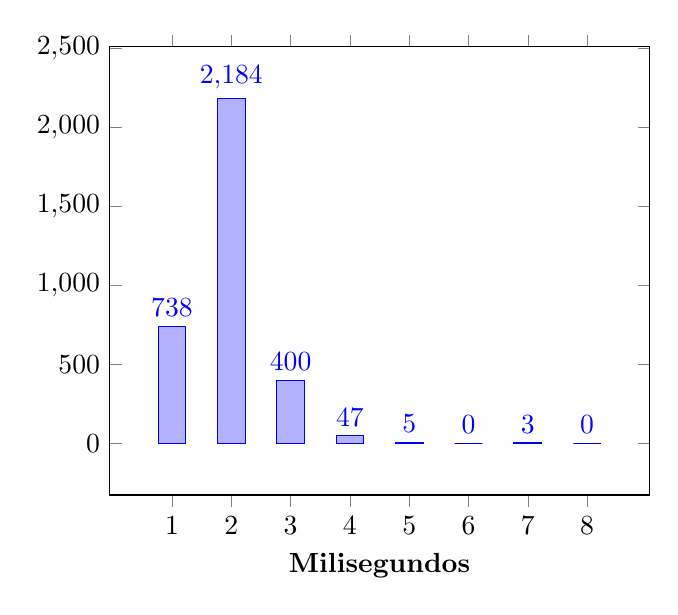
\begin{tikzpicture}
\begin{axis}[
    ybar,
    enlargelimits=0.15,
    legend style={at={(0.5,-0.15)},
    anchor=north,legend columns=-1},
    xlabel={\textbf{Milisegundos}},
    symbolic x coords={1,2,3,4,5,6,7,8},
    xtick=data,
    nodes near coords,
    nodes near coords align={vertical},
    ]
\addplot coordinates {(1,738) (2,2184) (3,400) (4,47) (5,5) (6,0) (7,3) (8,0)};
\end{axis}
\end{tikzpicture}
}%
\caption{Tiempo de descompresi\'on PNG en dispositivo Android Usuario 1}
\end{figure}

\begin{figure}[!h]
\centering
\resizebox{0.5\textwidth}{!}{%
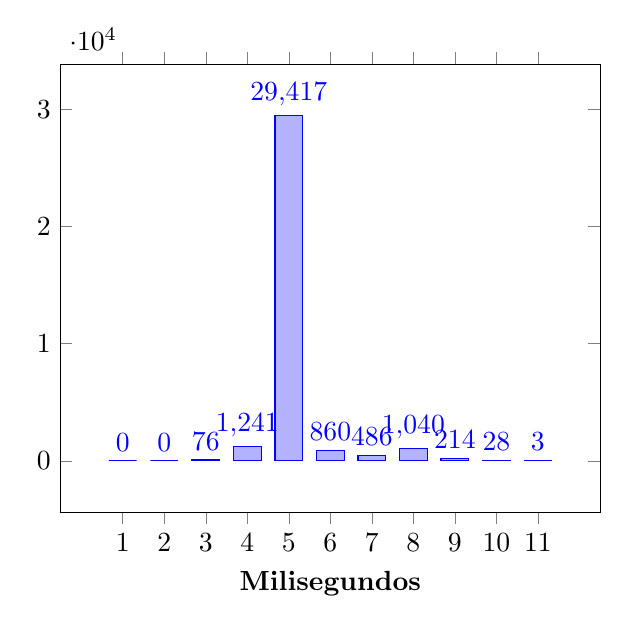
\begin{tikzpicture}
\begin{axis}[
    ybar,
    enlargelimits=0.15,
    legend style={at={(0.5,-0.15)},
    anchor=north,legend columns=-1},
    xlabel={\textbf{Milisegundos}},
    symbolic x coords={1,2,3,4,5,6,7,8,9,10,11},
    xtick=data,
    nodes near coords,
    nodes near coords align={vertical},
    ]
\addplot coordinates {(1,0) (2,0) (3,76) (4,1241) (5,29417) (6,860) (7,486) (8,1040) (9,214) (10,28) (11,3)};
\end{axis}
\end{tikzpicture}
}%
\caption{Tiempo de conversi\'on de c\'arama de Unity a PNG Usuario 1}
\end{figure}

Con los dispositivos utilizados se obtiene una media en milisegundos de descompresi\'on de PNG de XX y de transformaci\'on de textura de Unity a PNG de XX. La moda en la descompresi\'on del PNG es de 2 milisegundos y la moda en el tiempo de conversi\'on de textura a PNG es de 5 milisegundos. Sumado a esto tenemos los 2 milisegundos de latencia por lo que el proceso completo estar\'ia en los 9 milisegundos en la mayor\'ia de los casos. El umbral en el que el ojo humano detecta un cambio en las im\'agenes es de 14 milisegundos por lo que al encontrarse por debajo podemos asegurar que la fluidez durante la sesi\'on fue la \'optima.
%---------------------------------------------------------------------
%---------------------------------------------------------------------
%---------------------------------------------------------------------
%---------------------------------------------------------------------

\newpage \item \textbf{Usuario 2}

Este usuario tiene 23 a\~nos y es un jugador habitual. Suele jugar a juegos como Call Of Duty: MW, Dragalia Lost y Mario Kart 8.
Las pruebas se han realizado con los siguientes dispositivos: \\

\begin{tabularx}{1.0\textwidth} { 
  | >{\centering\arraybackslash}X 
  | >{\centering\arraybackslash}X 
  | >{\centering\arraybackslash}X 
  | >{\centering\arraybackslash}X | }
 \hline
 \textbf{Tarjeta Gr\'afica} & \textbf{Procesador} & \textbf{RAM} & \textbf{Modelo M\'ovil} \\
 \hline
 NVIDIA GeForce GTX 1080  &Intel(R) Core(TM) i7-6700K CPU @ 4.00GHz  & 16327 MB & One plus 6  \\
\hline
\end{tabularx}


Se han recogido los diferentes tiempos que tarda Unity en convertir la imagen que se optiene de la c\'amara a formato PNG, enviarse por red al dispositivo Android y el tiempo que este tarda en descomprimir el PNG y mostrar la imagen en la pantalla. 

Este usuario coment\'o durante la prueba que la vibraci\'on durante los derrapes era intermitente en vez de mantenida. Esto le desagrad\'o. En cuanto a si la experiencia fue fluida, el usuario contest\'o un 8 sobre 8 siendo 1 - Nada fluida y 8 - Completamente fluida. Cabe destacar que la latencia de red en el momento de la prueba era de 3 milisegundos.

\begin{figure}[!h]
\centering
\resizebox{0.5\textwidth}{!}{%
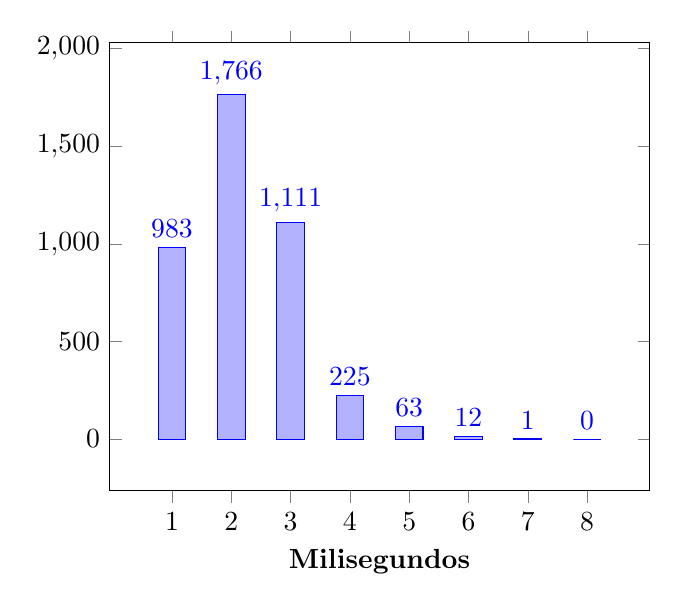
\begin{tikzpicture}
\begin{axis}[
    ybar,
    enlargelimits=0.15,
    legend style={at={(0.5,-0.15)},
    anchor=north,legend columns=-1},
    xlabel={\textbf{Milisegundos}},
    symbolic x coords={1,2,3,4,5,6,7,8},
    xtick=data,
    nodes near coords,
    nodes near coords align={vertical},
    ]
\addplot coordinates {(1,983) (2,1766) (3,1111) (4,225) (5,63) (6,12) (7,1) (8,0)};
\end{axis}
\end{tikzpicture}
}%
\caption{Tiempo de descompresi\'on PNG en dispositivo Android Usuario 2}
\end{figure}

\begin{figure}[!h]
\centering
\resizebox{0.5\textwidth}{!}{%
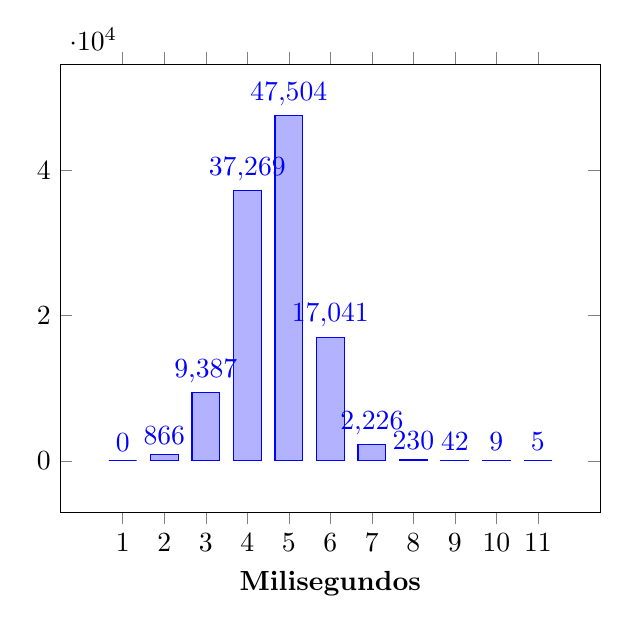
\begin{tikzpicture}
\begin{axis}[
    ybar,
    enlargelimits=0.15,
    legend style={at={(0.5,-0.15)},
    anchor=north,legend columns=-1},
    xlabel={\textbf{Milisegundos}},
    symbolic x coords={1,2,3,4,5,6,7,8,9,10,11},
    xtick=data,
    nodes near coords,
    nodes near coords align={vertical},
    ]
\addplot coordinates {(1,0) (2,866) (3,9387) (4,37269) (5,47504) (6,17041) (7,2226) (8,230) (9,42) (10,9) (11,5)};
\end{axis}
\end{tikzpicture}
}%
\caption{Tiempo de conversi\'on de c\'arama de Unity a PNG Usuario 2}
\end{figure}

Con los dispositivos utilizados se obtiene una media en milisegundos de descompresi\'on de PNG de XX y de transformaci\'on de textura de Unity a PNG de XX. La moda en la descompresi\'on del PNG es de 2-3 milisegundos y la moda en el tiempo de conversi\'on de textura a PNG es de 4 y 5 milisegundos la mayor parte de las veces. Sumado a esto tenemos los 3 milisegundos de latencia por lo que el proceso completo estar\'ia entre 9-11 milisegundos en la mayor\'ia de los casos. El umbral en el que el ojo humano detecta un cambio en las im\'agenes es de 14 milisegundos por lo que al encontrarse por debajo podemos asegurar que la fluidez durante la sesi\'on fue la \'optima.

%---------------------------------------------------------------------
%---------------------------------------------------------------------
%---------------------------------------------------------------------
%---------------------------------------------------------------------
\item \textbf{Usuario 3}

Este usuario tiene 49 a\~nos y es un jugador casual. Suele jugar a juegos como Age of Empires, Destiny, ARK y La Batalla por la Tierra Miedia.
Las pruebas se han realizado con los siguientes dispositivos: \\

\begin{tabularx}{1.0\textwidth} { 
  | >{\centering\arraybackslash}X 
  | >{\centering\arraybackslash}X 
  | >{\centering\arraybackslash}X 
  | >{\centering\arraybackslash}X | }
 \hline
 \textbf{Tarjeta Gr\'afica} & \textbf{Procesador} & \textbf{RAM} & \textbf{Modelo M\'ovil} \\
 \hline
 NVIDIA GeForce GTX 960M  & Intel(R) Core(TM) i7-6700HQ CPU @ 2.60GHz  & 16289 MB & Samsung Galaxy S9+  \\
\hline
\end{tabularx}


Se han recogido los diferentes tiempos que tarda Unity en convertir la imagen que se optiene de la c\'amara a formato PNG, enviarse por red al dispositivo Android y el tiempo que este tarda en descomprimir el PNG y mostrar la imagen en la pantalla. 

Este usuario coment\'o durante la prueba que la vibraci\'on era demasiado fuerte por lo que deber\'ia de disminuir la intensidad. Esto le desagrad\'o. En cuanto a si la experiencia fue fluida, el usuario contest\'o un 5 sobre 8 siendo 1 - Nada fluida y 8 - Completamente fluida. Cabe destacar que la latencia de red en el momento de la prueba era de 2 milisegundos.

\begin{figure}[!h]
\centering
\resizebox{0.5\textwidth}{!}{%
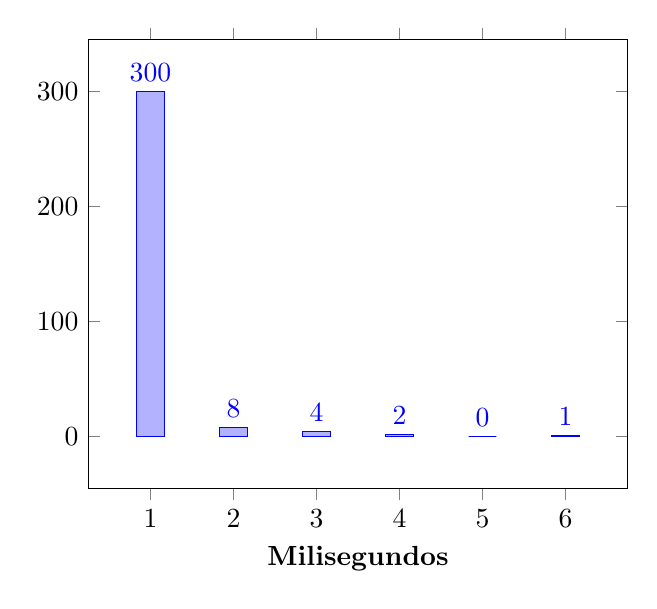
\begin{tikzpicture}
\begin{axis}[
    ybar,
    enlargelimits=0.15,
    legend style={at={(0.5,-0.15)},
    anchor=north,legend columns=-1},
    xlabel={\textbf{Milisegundos}},
    symbolic x coords={1,2,3,4,5,6},
    xtick=data,
    nodes near coords,
    nodes near coords align={vertical},
    ]
\addplot coordinates {(1,300) (2,8) (3,4) (4,2) (5,0) (6,1)};
\end{axis}
\end{tikzpicture}
}%
\caption{Tiempo de descompresi\'on PNG en dispositivo Android Usuario 3}
\end{figure}

\begin{figure}[!h]
\centering
\resizebox{0.5\textwidth}{!}{%
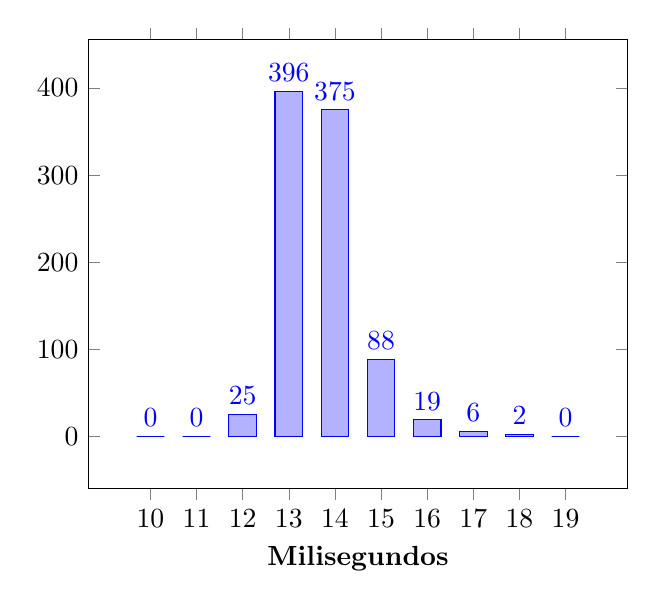
\begin{tikzpicture}
\begin{axis}[
    ybar,
    enlargelimits=0.15,
    legend style={at={(0.5,-0.15)},
    anchor=north,legend columns=-1},
    xlabel={\textbf{Milisegundos}},
    symbolic x coords={10,11,12,13,14,15,16,17,18,19},
    xtick=data,
    nodes near coords,
    nodes near coords align={vertical},
    ]
\addplot coordinates {(10,0) (11,0) (12,25) (13,396) (14,375) (15,88) (16,19) (17,6) (18,2) (19,0)};
\end{axis}
\end{tikzpicture}
}%
\caption{Tiempo de conversi\'on de c\'arama de Unity a PNG Usuario 3}
\end{figure}

Con los dispositivos utilizados se obtiene una media en milisegundos de descompresi\'on de PNG de XX y de transformaci\'on de textura de Unity a PNG de XX. La moda en la descompresi\'on del PNG es de 1 milisegundos y la moda en el tiempo de conversi\'on de textura a PNG es de 13 y 14 milisegundos la mayor parte de las veces. Sumado a esto tenemos los 2 milisegundos de latencia por lo que el proceso completo estar\'ia entre 16 y 17 milisegundos en la mayor\'ia de los casos. El umbral en el que el ojo humano detecta un cambio en las im\'agenes es de 14 milisegundos por lo que al encontrarse por encima la fluidez no ha sido la \'optima.

%---------------------------------------------------------------------
%---------------------------------------------------------------------
%---------------------------------------------------------------------
%---------------------------------------------------------------------

\item \textbf{Usuario 4}

Este usuario tiene 51 a\~nos y no juega a videojuegos salvo en momentos muy concretos. Los juegos a los que ha jugado en alg\'un momento han sido Mario Kart de Wii y Scrabble para Android.
Las pruebas se han realizado con los siguientes dispositivos: \\

\begin{tabularx}{1.0\textwidth} { 
  | >{\centering\arraybackslash}X 
  | >{\centering\arraybackslash}X 
  | >{\centering\arraybackslash}X 
  | >{\centering\arraybackslash}X | }
 \hline
 \textbf{Tarjeta Gr\'afica} & \textbf{Procesador} & \textbf{RAM} & \textbf{Modelo M\'ovil} \\
 \hline
AMD Radeon HD 7660D  & AMD A10-5800K APU with Radeon(tm) HD Graphics  & 7367 MB & Samsung Galaxy S8  \\
\hline
\end{tabularx}


Se han recogido los diferentes tiempos que tarda Unity en convertir la imagen que se optiene de la c\'amara a formato PNG, enviarse por red al dispositivo Android y el tiempo que este tarda en descomprimir el PNG y mostrar la imagen en la pantalla. 

Este usuario coment\'o durante la prueba que los botones no se correspond\'ian por completo con los mostrados en la imagen, ten\'ia que pulsar un poco fuera del bot\'on para que este se detectase. En cuanto a si la experiencia fue fluida, el usuario contest\'o un 7 sobre 8 siendo 1 - Nada fluida y 8 - Completamente fluida. Cabe destacar que la latencia de red en el momento de la prueba era de 2 milisegundos.

\begin{figure}[!h]
\centering
\resizebox{0.5\textwidth}{!}{%
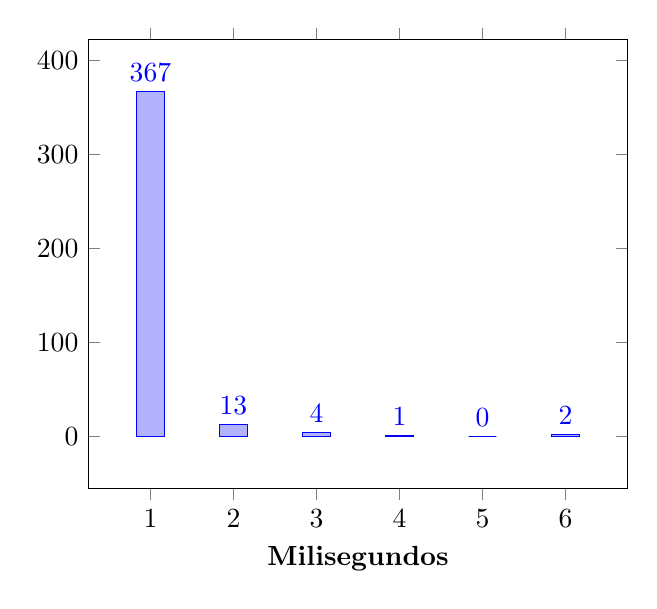
\begin{tikzpicture}
\begin{axis}[
    ybar,
    enlargelimits=0.15,
    legend style={at={(0.5,-0.15)},
    anchor=north,legend columns=-1},
    xlabel={\textbf{Milisegundos}},
    symbolic x coords={1,2,3,4,5,6},
    xtick=data,
    nodes near coords,
    nodes near coords align={vertical},
    ]
\addplot coordinates {(1,367) (2,13) (3,4) (4,1) (5,0) (6,2)};
\end{axis}
\end{tikzpicture}
}%
\caption{Tiempo de descompresi\'on PNG en dispositivo Android Usuario 4}
\end{figure}

\begin{figure}[!h]
\centering
\resizebox{0.5\textwidth}{!}{%
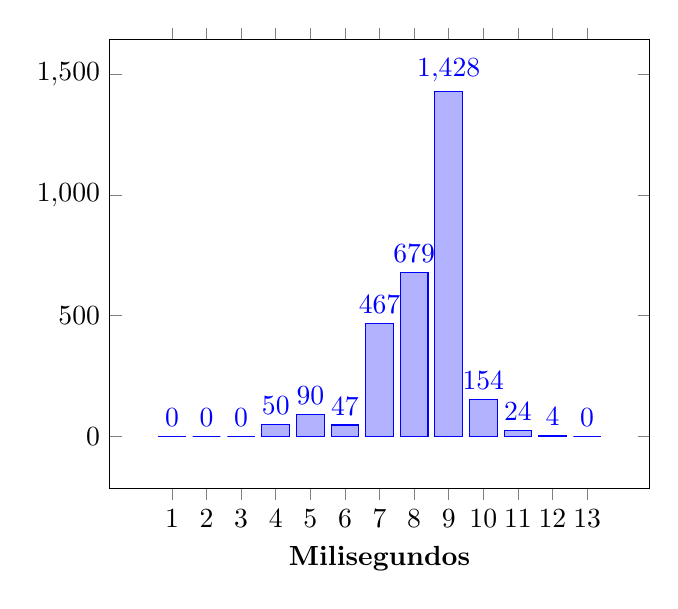
\begin{tikzpicture}
\begin{axis}[
    ybar,
    enlargelimits=0.15,
    legend style={at={(0.5,-0.15)},
    anchor=north,legend columns=-1},
    xlabel={\textbf{Milisegundos}},
    symbolic x coords={1,2,3,4,5,6,7,8,9,10,11,12,13},
    xtick=data,
    nodes near coords,
    nodes near coords align={vertical},
    ]
\addplot coordinates  {(1,0) (2,0) (3,0) (4,50) (5,90) (6,47) (7,467) (8,679) (9,1428) (10,154) (11,24) (12,4) (13,0) };
\end{axis}
\end{tikzpicture}
}%
\caption{Tiempo de conversi\'on de c\'arama de Unity a PNG Usuario 4}
\end{figure}

Con los dispositivos utilizados se obtiene una media en milisegundos de descompresi\'on de PNG de XX y de transformaci\'on de textura de Unity a PNG de XX. La moda en la descompresi\'on del PNG es de 1 milisegundos y la moda en el tiempo de conversi\'on de textura a PNG es de 7-9 milisegundos la mayor parte de las veces. Sumado a esto tenemos los 2 milisegundos de latencia por lo que el proceso completo estar\'ia entre 10-12 milisegundos en la mayor\'ia de los casos. El umbral en el que el ojo humano detecta un cambio en las im\'agenes es de 14 milisegundos por lo que al encontrarse por debajo podemos asegurar que la fluidez durante la sesi\'on fue la \'optima.

%---------------------------------------------------------------------
%---------------------------------------------------------------------
%---------------------------------------------------------------------
%---------------------------------------------------------------------

\item \textbf{Usuario 5}

Este usuario tiene 19 a\~nos y es un jugador habitual de juegos en todas las plataformas actuales (PC, PS4, Switch y Android). Los juegos a los que suele jugar son World Of Warcraft, The Legend of Zelda, Mario Kart, Total War y Assassin's Creed.
Las pruebas se han realizado con los siguientes dispositivos: \\

\begin{tabularx}{1.0\textwidth} { 
  | >{\centering\arraybackslash}X 
  | >{\centering\arraybackslash}X 
  | >{\centering\arraybackslash}X 
  | >{\centering\arraybackslash}X | }
 \hline
 \textbf{Tarjeta Gr\'afica} & \textbf{Procesador} & \textbf{RAM} & \textbf{Modelo M\'ovil} \\
 \hline
NVIDIA GeForce GTX 1080  & Intel(R) Core(TM) i7-6800K CPU @ 3.40GHz  & 32668 MB & Samsung Galaxy S9+  \\
\hline
\end{tabularx}


Se han recogido los diferentes tiempos que tarda Unity en convertir la imagen que se optiene de la c\'amara a formato PNG, enviarse por red al dispositivo Android y el tiempo que este tarda en descomprimir el PNG y mostrar la imagen en la pantalla. 

Este usuario coment\'o durante la prueba que los botones no se correspond\'ian por completo con los mostrados en la imagen, ten\'ia que pulsar un poco fuera del bot\'on para que este se detectase. En cuanto a si la experiencia fue fluida, el usuario contest\'o un 7 sobre 8 siendo 1 - Nada fluida y 8 - Completamente fluida. Cabe destacar que la latencia de red en el momento de la prueba era de 1 milisegundos.

\begin{figure}[!h]
\centering
\resizebox{0.5\textwidth}{!}{%
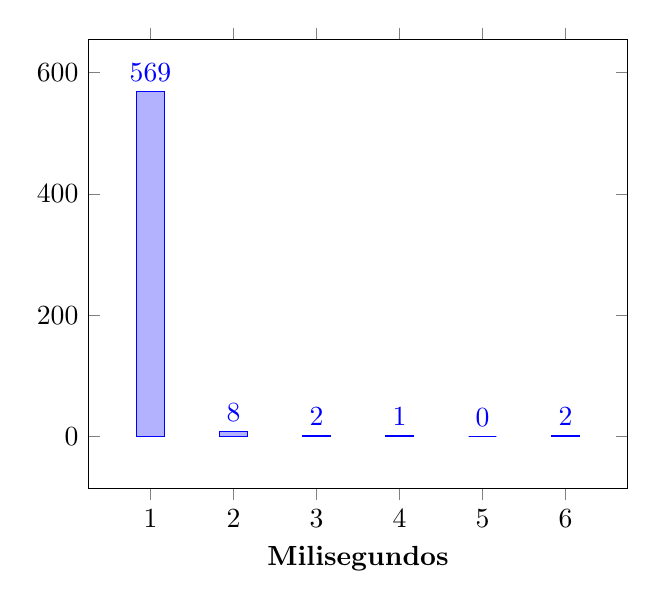
\begin{tikzpicture}
\begin{axis}[
    ybar,
    enlargelimits=0.15,
    legend style={at={(0.5,-0.15)},
    anchor=north,legend columns=-1},
    xlabel={\textbf{Milisegundos}},
    symbolic x coords={1,2,3,4,5,6},
    xtick=data,
    nodes near coords,
    nodes near coords align={vertical},
    ]
\addplot coordinates {(1,569) (2,8) (3,2) (4,1) (5,0) (6,2)};
\end{axis}
\end{tikzpicture}
}%
\caption{Tiempo de descompresi\'on PNG en dispositivo Android Usuario 5}
\end{figure}

\begin{figure}[!h]
\centering
\resizebox{0.5\textwidth}{!}{%
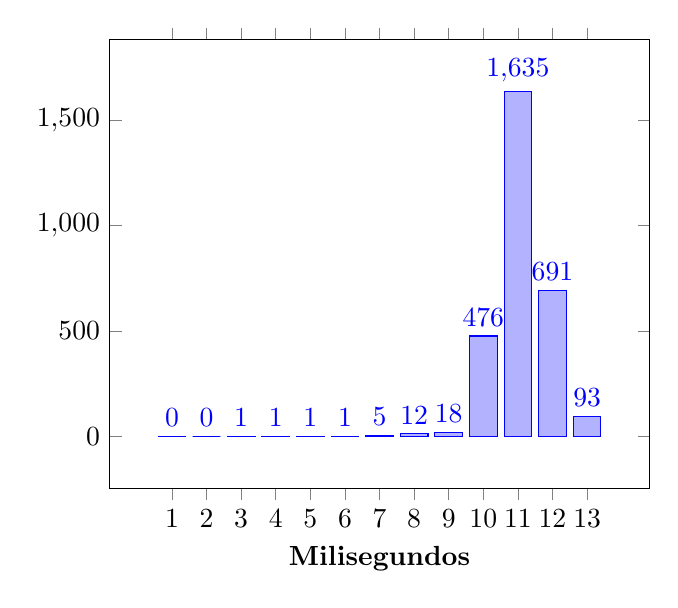
\begin{tikzpicture}
\begin{axis}[
    ybar,
    enlargelimits=0.15,
    legend style={at={(0.5,-0.15)},
    anchor=north,legend columns=-1},
    xlabel={\textbf{Milisegundos}},
    symbolic x coords={1,2,3,4,5,6,7,8,9,10,11,12,13,14,15,16},
    xtick=data,
    nodes near coords,
    nodes near coords align={vertical},
    ]
\addplot coordinates  {(1,0) (2,0) (3,1) (4,1) (5,1) (6,1) (7,5) (8,12) (9,18) (10,476) (11,1635) (12,691) (13,93) };
\end{axis}
\end{tikzpicture}
}%
\caption{Tiempo de conversi\'on de c\'arama de Unity a PNG Usuario 5}
\end{figure}

Con los dispositivos utilizados se obtiene una media en milisegundos de descompresi\'on de PNG de XX y de transformaci\'on de textura de Unity a PNG de XX. La moda en la descompresi\'on del PNG es de 1 milisegundos y la moda en el tiempo de conversi\'on de textura a PNG es de 10-12 milisegundos la mayor parte de las veces. Sumado a esto tenemos los 1 milisegundos de latencia por lo que el proceso completo estar\'ia entre 12-14 milisegundos en la mayor\'ia de los casos. El umbral en el que el ojo humano detecta un cambio en las im\'agenes es de 14 milisegundos por lo que al encontrarse por debajo podemos asegurar que la fluidez durante la sesi\'on fue la \'optima.

%---------------------------------------------------------------------
%---------------------------------------------------------------------
%---------------------------------------------------------------------
%---------------------------------------------------------------------

\end{enumerate}


% Variable local para emacs, para  que encuentre el fichero maestro de
% compilaci�n y funcionen mejor algunas teclas r�pidas de AucTeX
%%%
%%% Local Variables:
%%% mode: latex
%%% TeX-master: "../ManualTeXiS.tex"
%%% End:


\chapter{Conclusiones y trabajo futuro}
\label{cap7}
\label{cap:conclusiones}


El objetivo de este proyecto era el de utilizar un dispositivo m\'ovil como dispositivo de entrada para videojuegos. Para conseguir esto, se ha realizado una librer\'ia aplicable en el motor de videojuegos Unity con el objetivo de poder utilizar un dispositivo m\'ovil como dispositivo de entrada durante una sesi\'on de juego. Posterior al desarrollo de la librer\'ia, se ha ralizado una implementaci\'on en un juego terminado con la que realizar pruebas de rendimiento de la herramienta.\\

El resultado de estas pruebas mostraron que la librer\'ia se comporta como se esperaba y que alcanza la tasa de fotogramas por segundo m\'inima aceptable en diferentes dispositivos. Estos resultados dejaron claro que el rendimiento de la librer\'ia est\'a ligado al \textit{hardware} donde se est\'a ejecutando. En los pr\'oximos p\'arrafos se expondr\'an diferentes posibles mejoras para el proyecto.\\

Existen diferentes algoritmos de compresi\'on de im\'agenes y en este proyecto se ha utilizado PNG debido a que se encuentra integrado en las dos plataformas utilizadas durante el desarrollo de la librer\'ia. Este formato de compresi\'on de im\'agenes es m\'as r\'apido cuanto menor sea la variedad de colores que contenga la im\'agen. En el videojuego utilizado para la prueba con usuarios, la im\'agen que se enviaba al dispositivo m\'ovil ten\'ia siempre los mismos colores, es por esto que el uso del formato PNG era suficiente. Para conseguir que los resultados sean mejores con im\'agenes m\'as complejas, se propone la b\'usqueda de un m\'etodo de compresi\'on de im\'agenes alternativo.\\

El uso de un m\'ovil como dispositivo de entrada no solo aporta una pantalla t\'actil en la que poder tener un mando, adem\'as de esto pueden utilizarse los diferentes sensores con los que cuentan estos dispositivos. Los sensores a los que se quiere dar m\'as importancia en este proyecto son el aceler\'ometro y el giroscopio. Estos sensores no se encuentran \'unicamente en los m\'oviles sino que tambi\'en se encuentran en otros dispositivos de entrada de algunas consolas antiguas. Por falta de tiempo, no se pudo implementar la monitorizaci\'on de estos sensores para ser utilizados en la librer\'ia pero su inclusi\'on dar\'ia m\'as versatilidad al desarrollador.\\

Por falta de tiempo durante el desarrollo de este trabajo, se abandon\'o la idea de permitir el uso de m\'ultiples m\'oviles durante una misma ejecuci\'on. Los juegos multijugador locales permitir\'ian exprimir al m\'aximo el uso de varios dispositivos m\'oviles, tal y como se hace en la saga de juegos PlayLink. Para conseguir esto es necesario la modificaci\'on del servidor de Unity para soportar m\'as de un cliente. \\

Adem\'as de lo relacionado con el apartado t\'ecnico del proyecto, un punto destacable a mejorar es el n\'umero de usuarios utilizado para las pruebas. Debido a la situaci\'on actual, las pruebas han tenido que realizarse en remoto, lo que hace que se necesite mucho m\'as tiempo para cada una de las pruebas. Con un cuestionario m\'as extenso y un n\'umero de usuarios mayor se podr\'ian dar valores estad\'isticos m\'as precisos. Con ello podr\'ian sacarse conclusiones con un peso estad\'istico mayor y tener una visi\'on m\'as global del rendimiento de la librer\'ia.

% Ap�ndices
%\appendix
%\include{Apendices/ParteApendices}
%\include{Apendices/01AsiSeHizo}

\backmatter

%
% Bibliograf�a
%

\bibliography{sample}

%
% �ndice de palabras
%

\ifx\generaindice\undefined
\else
\include{TeXiS/TeXiS_indice}
\fi

%
% Lista de acr�nimos
%

% S�lo  lo  generamos  si  est� declarada  \generaacronimos.  Consulta
% TeXiS.sty para m�s informaci�n.


\ifx\generaacronimos\undefined
\else
%\include{TeXiS/TeXiS_acron}
\fi

%
% Final
%%
%\include{Cascaras/fin}

\end{document}
